\batchmode
\documentclass[twoside]{book}

% Packages required by doxygen
\usepackage{fixltx2e}
\usepackage{calc}
\usepackage{doxygen}
\usepackage[export]{adjustbox} % also loads graphicx
\usepackage{graphicx}
\usepackage[utf8]{inputenc}
\usepackage{makeidx}
\usepackage{multicol}
\usepackage{multirow}
\PassOptionsToPackage{warn}{textcomp}
\usepackage{textcomp}
\usepackage[nointegrals]{wasysym}
\usepackage[table]{xcolor}

% Font selection
\usepackage[T1]{fontenc}
\usepackage[scaled=.90]{helvet}
\usepackage{courier}
\usepackage{amssymb}
\usepackage{sectsty}
\renewcommand{\familydefault}{\sfdefault}
\allsectionsfont{%
  \fontseries{bc}\selectfont%
  \color{darkgray}%
}
\renewcommand{\DoxyLabelFont}{%
  \fontseries{bc}\selectfont%
  \color{darkgray}%
}
\newcommand{\+}{\discretionary{\mbox{\scriptsize$\hookleftarrow$}}{}{}}

% Page & text layout
\usepackage{geometry}
\geometry{%
  a4paper,%
  top=2.5cm,%
  bottom=2.5cm,%
  left=2.5cm,%
  right=2.5cm%
}
\tolerance=750
\hfuzz=15pt
\hbadness=750
\setlength{\emergencystretch}{15pt}
\setlength{\parindent}{0cm}
\setlength{\parskip}{3ex plus 2ex minus 2ex}
\makeatletter
\renewcommand{\paragraph}{%
  \@startsection{paragraph}{4}{0ex}{-1.0ex}{1.0ex}{%
    \normalfont\normalsize\bfseries\SS@parafont%
  }%
}
\renewcommand{\subparagraph}{%
  \@startsection{subparagraph}{5}{0ex}{-1.0ex}{1.0ex}{%
    \normalfont\normalsize\bfseries\SS@subparafont%
  }%
}
\makeatother

% Headers & footers
\usepackage{fancyhdr}
\pagestyle{fancyplain}
\fancyhead[LE]{\fancyplain{}{\bfseries\thepage}}
\fancyhead[CE]{\fancyplain{}{}}
\fancyhead[RE]{\fancyplain{}{\bfseries\leftmark}}
\fancyhead[LO]{\fancyplain{}{\bfseries\rightmark}}
\fancyhead[CO]{\fancyplain{}{}}
\fancyhead[RO]{\fancyplain{}{\bfseries\thepage}}
\fancyfoot[LE]{\fancyplain{}{}}
\fancyfoot[CE]{\fancyplain{}{}}
\fancyfoot[RE]{\fancyplain{}{\bfseries\scriptsize Generated by Doxygen }}
\fancyfoot[LO]{\fancyplain{}{\bfseries\scriptsize Generated by Doxygen }}
\fancyfoot[CO]{\fancyplain{}{}}
\fancyfoot[RO]{\fancyplain{}{}}
\renewcommand{\footrulewidth}{0.4pt}
\renewcommand{\chaptermark}[1]{%
  \markboth{#1}{}%
}
\renewcommand{\sectionmark}[1]{%
  \markright{\thesection\ #1}%
}

% Indices & bibliography
\usepackage{natbib}
\usepackage[titles]{tocloft}
\setcounter{tocdepth}{3}
\setcounter{secnumdepth}{5}
\makeindex

% Hyperlinks (required, but should be loaded last)
\usepackage{ifpdf}
\ifpdf
  \usepackage[pdftex,pagebackref=true]{hyperref}
\else
  \usepackage[ps2pdf,pagebackref=true]{hyperref}
\fi
\hypersetup{%
  colorlinks=true,%
  linkcolor=blue,%
  citecolor=blue,%
  unicode%
}

% Custom commands
\newcommand{\clearemptydoublepage}{%
  \newpage{\pagestyle{empty}\cleardoublepage}%
}

\usepackage{caption}
\captionsetup{labelsep=space,justification=centering,font={bf},singlelinecheck=off,skip=4pt,position=top}

%===== C O N T E N T S =====

\begin{document}

% Titlepage & ToC
\hypersetup{pageanchor=false,
             bookmarksnumbered=true,
             pdfencoding=unicode
            }
\pagenumbering{alph}
\pagenumbering{arabic}
\hypersetup{pageanchor=true}

%--- Begin generated contents ---
\chapter{Example problem\+: Steady 2D finite-\/\+Reynolds-\/number flow in a channel of non-\/uniform width -\/-\/ An introduction to Spine meshes.}
\label{index}\hypertarget{index}{}\hypertarget{index_q}{}\section{A few quick questions...}\label{index_q}
Since {\ttfamily oomph-\/lib} is developed as open-\/source software, any evidence that the code is being downloaded and used is very helpful for us as it helps to justify our continued work on this project.

We would therefore be extremely grateful if you could provide the information requested in the form below. Pressing the \char`\"{}submit\char`\"{} button will get you to the actual download page.

{\bfseries Note\+:} 
\begin{DoxyItemize}
\item All information will be treated as confidential. 
\item If you provide your email address and check the appropriate box we will add you to our mailing list to inform you of upgrades and bug fixes to the code. Rest assured that the mailing list is {\bfseries very low volume} -- we have better things to do than to bombard you with email. 
\item If you still feel reluctant to provide any of the information requested, feel free to enter some dummy input. The form will check that {\bfseries some} information has been entered but entering your name as \char`\"{}\+Joe Cool\char`\"{} is perfectly acceptable -- this is to discourage people from not providing the information simply because they are too lazy to type... 
\end{DoxyItemize}



 







 

 \hypertarget{index_pdf}{}\section{P\+D\+F file}\label{index_pdf}
A \href{../latex/refman.pdf}{\tt pdf version} of this document is available. \end{document}

\chapter{Namespace Index}
\section{Namespace List}
Here is a list of all namespaces with brief descriptions\+:\begin{DoxyCompactList}
\item\contentsline{section}{\hyperlink{namespaceGlobal__Physical__Variables}{Global\+\_\+\+Physical\+\_\+\+Variables} \\*Global variables that represent physical properties }{\pageref{namespaceGlobal__Physical__Variables}}{}
\item\contentsline{section}{\hyperlink{namespaceoomph}{oomph} }{\pageref{namespaceoomph}}{}
\item\contentsline{section}{\hyperlink{namespacePhysical__Variables}{Physical\+\_\+\+Variables} \\*Namespace for the solution of 2D linear shell equation }{\pageref{namespacePhysical__Variables}}{}
\end{DoxyCompactList}

\chapter{Hierarchical Index}
\section{Class Hierarchy}
This inheritance list is sorted roughly, but not completely, alphabetically\+:\begin{DoxyCompactList}
\item Problem\begin{DoxyCompactList}
\item \contentsline{section}{Unstructured\+Solid\+Problem$<$ E\+L\+E\+M\+E\+NT $>$}{\pageref{classUnstructuredSolidProblem}}{}
\end{DoxyCompactList}
\end{DoxyCompactList}

\chapter{Class Index}
\section{Class List}
Here are the classes, structs, unions and interfaces with brief descriptions\+:\begin{DoxyCompactList}
\item\contentsline{section}{\hyperlink{classPMLProblem}{P\+M\+L\+Problem$<$ E\+L\+E\+M\+E\+N\+T $>$} }{\pageref{classPMLProblem}}{}
\item\contentsline{section}{\hyperlink{classGlobalParameters_1_1TestPMLMapping}{Global\+Parameters\+::\+Test\+P\+M\+L\+Mapping} }{\pageref{classGlobalParameters_1_1TestPMLMapping}}{}
\end{DoxyCompactList}

\chapter{File Index}
\section{File List}
Here is a list of all files with brief descriptions\+:\begin{DoxyCompactList}
\item\contentsline{section}{\hyperlink{jeffery__orbit_8cc}{jeffery\+\_\+orbit.\+cc} }{\pageref{jeffery__orbit_8cc}}{}
\item\contentsline{section}{\hyperlink{jeffery__orbit_8txt__doxygenified_8h}{jeffery\+\_\+orbit.\+txt\+\_\+doxygenified.\+h} }{\pageref{jeffery__orbit_8txt__doxygenified_8h}}{}
\item\contentsline{section}{\hyperlink{my__taylor__hood__elements_8h}{my\+\_\+taylor\+\_\+hood\+\_\+elements.\+h} }{\pageref{my__taylor__hood__elements_8h}}{}
\end{DoxyCompactList}

\chapter{Namespace Documentation}
\hypertarget{namespaceGlobal__Physical__Variables}{}\section{Global\+\_\+\+Physical\+\_\+\+Variables Namespace Reference}
\label{namespaceGlobal__Physical__Variables}\index{Global\+\_\+\+Physical\+\_\+\+Variables@{Global\+\_\+\+Physical\+\_\+\+Variables}}


Namespace for physical parameters.  


\subsection*{Functions}
\begin{DoxyCompactItemize}
\item 
Vector$<$ double $>$ \hyperlink{namespaceGlobal__Physical__Variables_afae321364975eb56688ad13abc8ed6b7}{Gravity} (2)
\begin{DoxyCompactList}\small\item\em Gravity vector. \end{DoxyCompactList}\item 
void \hyperlink{namespaceGlobal__Physical__Variables_a87da705b8a46bed337cf5dbdd788b87b}{body\+\_\+force} (const double \&time, const Vector$<$ double $>$ \&x, Vector$<$ double $>$ \&result)
\begin{DoxyCompactList}\small\item\em Functional body force. \end{DoxyCompactList}\item 
void \hyperlink{namespaceGlobal__Physical__Variables_a9780d615ae07c4e00a436ab2973b54e6}{zero\+\_\+body\+\_\+force} (const double \&time, const Vector$<$ double $>$ \&x, Vector$<$ double $>$ \&result)
\begin{DoxyCompactList}\small\item\em Zero functional body force. \end{DoxyCompactList}\end{DoxyCompactItemize}
\subsection*{Variables}
\begin{DoxyCompactItemize}
\item 
double \hyperlink{namespaceGlobal__Physical__Variables_ab814e627d2eb5bc50318879d19ab16b9}{Re} =100
\begin{DoxyCompactList}\small\item\em Reynolds number. \end{DoxyCompactList}\item 
double \hyperlink{namespaceGlobal__Physical__Variables_ab1a845a672b4d74b304639a976dc65c6}{Re\+\_\+inv\+Fr} =100
\begin{DoxyCompactList}\small\item\em Reynolds/\+Froude number. \end{DoxyCompactList}\end{DoxyCompactItemize}


\subsection{Detailed Description}
Namespace for physical parameters. 

\subsection{Function Documentation}
\mbox{\Hypertarget{namespaceGlobal__Physical__Variables_a87da705b8a46bed337cf5dbdd788b87b}\label{namespaceGlobal__Physical__Variables_a87da705b8a46bed337cf5dbdd788b87b}} 
\index{Global\+\_\+\+Physical\+\_\+\+Variables@{Global\+\_\+\+Physical\+\_\+\+Variables}!body\+\_\+force@{body\+\_\+force}}
\index{body\+\_\+force@{body\+\_\+force}!Global\+\_\+\+Physical\+\_\+\+Variables@{Global\+\_\+\+Physical\+\_\+\+Variables}}
\subsubsection{\texorpdfstring{body\+\_\+force()}{body\_force()}}
{\footnotesize\ttfamily void Global\+\_\+\+Physical\+\_\+\+Variables\+::body\+\_\+force (\begin{DoxyParamCaption}\item[{const double \&}]{time,  }\item[{const Vector$<$ double $>$ \&}]{x,  }\item[{Vector$<$ double $>$ \&}]{result }\end{DoxyParamCaption})}



Functional body force. 



Definition at line 62 of file circular\+\_\+driven\+\_\+cavity.\+cc.



References Re\+\_\+inv\+Fr.



Referenced by main().

\mbox{\Hypertarget{namespaceGlobal__Physical__Variables_afae321364975eb56688ad13abc8ed6b7}\label{namespaceGlobal__Physical__Variables_afae321364975eb56688ad13abc8ed6b7}} 
\index{Global\+\_\+\+Physical\+\_\+\+Variables@{Global\+\_\+\+Physical\+\_\+\+Variables}!Gravity@{Gravity}}
\index{Gravity@{Gravity}!Global\+\_\+\+Physical\+\_\+\+Variables@{Global\+\_\+\+Physical\+\_\+\+Variables}}
\subsubsection{\texorpdfstring{Gravity()}{Gravity()}}
{\footnotesize\ttfamily Vector$<$double$>$ Global\+\_\+\+Physical\+\_\+\+Variables\+::\+Gravity (\begin{DoxyParamCaption}\item[{2}]{ }\end{DoxyParamCaption})}



Gravity vector. 



Referenced by main(), and Quarter\+Circle\+Driven\+Cavity\+Problem$<$ E\+L\+E\+M\+E\+N\+T $>$\+::\+Quarter\+Circle\+Driven\+Cavity\+Problem().

\mbox{\Hypertarget{namespaceGlobal__Physical__Variables_a9780d615ae07c4e00a436ab2973b54e6}\label{namespaceGlobal__Physical__Variables_a9780d615ae07c4e00a436ab2973b54e6}} 
\index{Global\+\_\+\+Physical\+\_\+\+Variables@{Global\+\_\+\+Physical\+\_\+\+Variables}!zero\+\_\+body\+\_\+force@{zero\+\_\+body\+\_\+force}}
\index{zero\+\_\+body\+\_\+force@{zero\+\_\+body\+\_\+force}!Global\+\_\+\+Physical\+\_\+\+Variables@{Global\+\_\+\+Physical\+\_\+\+Variables}}
\subsubsection{\texorpdfstring{zero\+\_\+body\+\_\+force()}{zero\_body\_force()}}
{\footnotesize\ttfamily void Global\+\_\+\+Physical\+\_\+\+Variables\+::zero\+\_\+body\+\_\+force (\begin{DoxyParamCaption}\item[{const double \&}]{time,  }\item[{const Vector$<$ double $>$ \&}]{x,  }\item[{Vector$<$ double $>$ \&}]{result }\end{DoxyParamCaption})}



Zero functional body force. 



Definition at line 70 of file circular\+\_\+driven\+\_\+cavity.\+cc.



Referenced by main().



\subsection{Variable Documentation}
\mbox{\Hypertarget{namespaceGlobal__Physical__Variables_ab814e627d2eb5bc50318879d19ab16b9}\label{namespaceGlobal__Physical__Variables_ab814e627d2eb5bc50318879d19ab16b9}} 
\index{Global\+\_\+\+Physical\+\_\+\+Variables@{Global\+\_\+\+Physical\+\_\+\+Variables}!Re@{Re}}
\index{Re@{Re}!Global\+\_\+\+Physical\+\_\+\+Variables@{Global\+\_\+\+Physical\+\_\+\+Variables}}
\subsubsection{\texorpdfstring{Re}{Re}}
{\footnotesize\ttfamily double Global\+\_\+\+Physical\+\_\+\+Variables\+::\+Re =100}



Reynolds number. 



Definition at line 53 of file circular\+\_\+driven\+\_\+cavity.\+cc.



Referenced by Quarter\+Circle\+Driven\+Cavity\+Problem$<$ E\+L\+E\+M\+E\+N\+T $>$\+::\+Quarter\+Circle\+Driven\+Cavity\+Problem().

\mbox{\Hypertarget{namespaceGlobal__Physical__Variables_ab1a845a672b4d74b304639a976dc65c6}\label{namespaceGlobal__Physical__Variables_ab1a845a672b4d74b304639a976dc65c6}} 
\index{Global\+\_\+\+Physical\+\_\+\+Variables@{Global\+\_\+\+Physical\+\_\+\+Variables}!Re\+\_\+inv\+Fr@{Re\+\_\+inv\+Fr}}
\index{Re\+\_\+inv\+Fr@{Re\+\_\+inv\+Fr}!Global\+\_\+\+Physical\+\_\+\+Variables@{Global\+\_\+\+Physical\+\_\+\+Variables}}
\subsubsection{\texorpdfstring{Re\+\_\+inv\+Fr}{Re\_invFr}}
{\footnotesize\ttfamily double Global\+\_\+\+Physical\+\_\+\+Variables\+::\+Re\+\_\+inv\+Fr =100}



Reynolds/\+Froude number. 



Definition at line 56 of file circular\+\_\+driven\+\_\+cavity.\+cc.



Referenced by body\+\_\+force(), and Quarter\+Circle\+Driven\+Cavity\+Problem$<$ E\+L\+E\+M\+E\+N\+T $>$\+::\+Quarter\+Circle\+Driven\+Cavity\+Problem().


\hypertarget{namespaceGlobal__Physical__Variables2}{}\section{Global\+\_\+\+Physical\+\_\+\+Variables2 Namespace Reference}
\label{namespaceGlobal__Physical__Variables2}\index{Global\+\_\+\+Physical\+\_\+\+Variables2@{Global\+\_\+\+Physical\+\_\+\+Variables2}}


Namespace for physical parameters.  


\subsection*{Variables}
\begin{DoxyCompactItemize}
\item 
double \hyperlink{namespaceGlobal__Physical__Variables2_afce617c1bd6726b29fa0e1f7c892a955}{Re} =100
\begin{DoxyCompactList}\small\item\em Reynolds number. \end{DoxyCompactList}\end{DoxyCompactItemize}


\subsection{Detailed Description}
Namespace for physical parameters. 

\subsection{Variable Documentation}
\mbox{\Hypertarget{namespaceGlobal__Physical__Variables2_afce617c1bd6726b29fa0e1f7c892a955}\label{namespaceGlobal__Physical__Variables2_afce617c1bd6726b29fa0e1f7c892a955}} 
\index{Global\+\_\+\+Physical\+\_\+\+Variables2@{Global\+\_\+\+Physical\+\_\+\+Variables2}!Re@{Re}}
\index{Re@{Re}!Global\+\_\+\+Physical\+\_\+\+Variables2@{Global\+\_\+\+Physical\+\_\+\+Variables2}}
\subsubsection{\texorpdfstring{Re}{Re}}
{\footnotesize\ttfamily double Global\+\_\+\+Physical\+\_\+\+Variables2\+::\+Re =100}



Reynolds number. 



Definition at line 52 of file spine\+\_\+channel2.\+cc.



Referenced by Spiked\+Channel\+Spine\+Flow\+Problem$<$ E\+L\+E\+M\+E\+N\+T $>$\+::\+Spiked\+Channel\+Spine\+Flow\+Problem().


\chapter{Class Documentation}
\hypertarget{classChannelSpineFlowProblem}{}\section{Channel\+Spine\+Flow\+Problem$<$ E\+L\+E\+M\+E\+NT $>$ Class Template Reference}
\label{classChannelSpineFlowProblem}\index{Channel\+Spine\+Flow\+Problem$<$ E\+L\+E\+M\+E\+N\+T $>$@{Channel\+Spine\+Flow\+Problem$<$ E\+L\+E\+M\+E\+N\+T $>$}}
Inheritance diagram for Channel\+Spine\+Flow\+Problem$<$ E\+L\+E\+M\+E\+NT $>$\+:\begin{figure}[H]
\begin{center}
\leavevmode
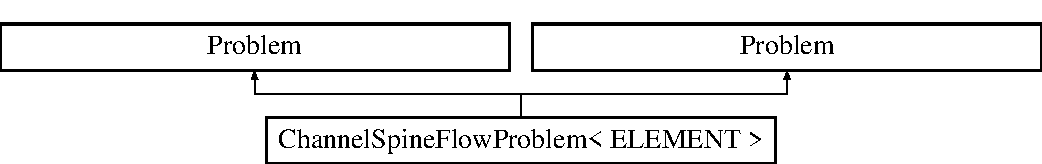
\includegraphics[height=2.000000cm]{classChannelSpineFlowProblem}
\end{center}
\end{figure}
\subsection*{Public Member Functions}
\begin{DoxyCompactItemize}
\item 
\hyperlink{classChannelSpineFlowProblem_a23f1b987e3395b1d101eaf3f3b5c94b2}{Channel\+Spine\+Flow\+Problem} ()
\begin{DoxyCompactList}\small\item\em Constructor. \end{DoxyCompactList}\item 
\hyperlink{classChannelSpineFlowProblem_abdf2cc520915167d8718499459df348b}{$\sim$\+Channel\+Spine\+Flow\+Problem} ()
\begin{DoxyCompactList}\small\item\em Destructor\+: (empty) \end{DoxyCompactList}\item 
void \hyperlink{classChannelSpineFlowProblem_aaf6dd8a8a472ccd938df579aba61ec97}{actions\+\_\+before\+\_\+newton\+\_\+solve} ()
\begin{DoxyCompactList}\small\item\em Update the problem specs before solve. Update the nodal positions. \end{DoxyCompactList}\item 
void \hyperlink{classChannelSpineFlowProblem_a419a80ef3d19438f193bd7843f72446a}{actions\+\_\+after\+\_\+newton\+\_\+solve} ()
\begin{DoxyCompactList}\small\item\em Update the after solve (empty) \end{DoxyCompactList}\item 
void \hyperlink{classChannelSpineFlowProblem_a101bdeee56502231945cbac272ca21f6}{doc\+\_\+solution} (Doc\+Info \&doc\+\_\+info)
\begin{DoxyCompactList}\small\item\em Doc the solution. \end{DoxyCompactList}\item 
\hyperlink{classSimpleSpineMesh}{Simple\+Spine\+Mesh}$<$ E\+L\+E\+M\+E\+NT $>$ $\ast$ \hyperlink{classChannelSpineFlowProblem_ab68c7ab5406b90a0ef56c39b67f83a09}{mesh\+\_\+pt} ()
\begin{DoxyCompactList}\small\item\em Overload access to mesh. \end{DoxyCompactList}\item 
\hyperlink{classChannelSpineFlowProblem_a23f1b987e3395b1d101eaf3f3b5c94b2}{Channel\+Spine\+Flow\+Problem} ()
\begin{DoxyCompactList}\small\item\em Constructor. \end{DoxyCompactList}\item 
\hyperlink{classChannelSpineFlowProblem_abdf2cc520915167d8718499459df348b}{$\sim$\+Channel\+Spine\+Flow\+Problem} ()
\begin{DoxyCompactList}\small\item\em Destructor\+: (empty) \end{DoxyCompactList}\item 
void \hyperlink{classChannelSpineFlowProblem_aaf6dd8a8a472ccd938df579aba61ec97}{actions\+\_\+before\+\_\+newton\+\_\+solve} ()
\begin{DoxyCompactList}\small\item\em Update the problem specs before solve. Set velocity boundary conditions just to be on the safe side... \end{DoxyCompactList}\item 
void \hyperlink{classChannelSpineFlowProblem_a419a80ef3d19438f193bd7843f72446a}{actions\+\_\+after\+\_\+newton\+\_\+solve} ()
\begin{DoxyCompactList}\small\item\em Update the after solve (empty) \end{DoxyCompactList}\item 
void \hyperlink{classChannelSpineFlowProblem_a101bdeee56502231945cbac272ca21f6}{doc\+\_\+solution} (Doc\+Info \&doc\+\_\+info)
\begin{DoxyCompactList}\small\item\em Doc the solution. \end{DoxyCompactList}\end{DoxyCompactItemize}
\subsection*{Private Attributes}
\begin{DoxyCompactItemize}
\item 
double \hyperlink{classChannelSpineFlowProblem_a6ac51c3c9d400869e694fe00452e293f}{Ly}
\begin{DoxyCompactList}\small\item\em Width of channel. \end{DoxyCompactList}\end{DoxyCompactItemize}


\subsection{Detailed Description}
\subsubsection*{template$<$class E\+L\+E\+M\+E\+NT$>$\newline
class Channel\+Spine\+Flow\+Problem$<$ E\+L\+E\+M\+E\+N\+T $>$}

Channel flow through a non-\/uniform channel whose geometry is defined by a spine mesh. 

Definition at line 462 of file simple\+\_\+spine\+\_\+channel.\+cc.



\subsection{Constructor \& Destructor Documentation}
\mbox{\Hypertarget{classChannelSpineFlowProblem_a23f1b987e3395b1d101eaf3f3b5c94b2}\label{classChannelSpineFlowProblem_a23f1b987e3395b1d101eaf3f3b5c94b2}} 
\index{Channel\+Spine\+Flow\+Problem@{Channel\+Spine\+Flow\+Problem}!Channel\+Spine\+Flow\+Problem@{Channel\+Spine\+Flow\+Problem}}
\index{Channel\+Spine\+Flow\+Problem@{Channel\+Spine\+Flow\+Problem}!Channel\+Spine\+Flow\+Problem@{Channel\+Spine\+Flow\+Problem}}
\subsubsection{\texorpdfstring{Channel\+Spine\+Flow\+Problem()}{ChannelSpineFlowProblem()}\hspace{0.1cm}{\footnotesize\ttfamily [1/2]}}
{\footnotesize\ttfamily template$<$class E\+L\+E\+M\+E\+NT $>$ \\
\hyperlink{classChannelSpineFlowProblem}{Channel\+Spine\+Flow\+Problem}$<$ E\+L\+E\+M\+E\+NT $>$\+::\hyperlink{classChannelSpineFlowProblem}{Channel\+Spine\+Flow\+Problem} (\begin{DoxyParamCaption}{ }\end{DoxyParamCaption})}



Constructor. 

Constructor for Channel\+Spine\+Flow problem. 

Definition at line 509 of file simple\+\_\+spine\+\_\+channel.\+cc.



References Global\+\_\+\+Physical\+\_\+\+Variables\+::H, Global\+\_\+\+Physical\+\_\+\+Variables\+::height(), Simple\+Spine\+Mesh$<$ E\+L\+E\+M\+E\+N\+T $>$\+::height\+\_\+fct\+\_\+pt(), Global\+\_\+\+Physical\+\_\+\+Variables\+::\+L\+\_\+total, and Global\+\_\+\+Physical\+\_\+\+Variables\+::\+Re.



Referenced by Channel\+Spine\+Flow\+Problem$<$ E\+L\+E\+M\+E\+N\+T $>$\+::actions\+\_\+after\+\_\+newton\+\_\+solve().

\mbox{\Hypertarget{classChannelSpineFlowProblem_abdf2cc520915167d8718499459df348b}\label{classChannelSpineFlowProblem_abdf2cc520915167d8718499459df348b}} 
\index{Channel\+Spine\+Flow\+Problem@{Channel\+Spine\+Flow\+Problem}!````~Channel\+Spine\+Flow\+Problem@{$\sim$\+Channel\+Spine\+Flow\+Problem}}
\index{````~Channel\+Spine\+Flow\+Problem@{$\sim$\+Channel\+Spine\+Flow\+Problem}!Channel\+Spine\+Flow\+Problem@{Channel\+Spine\+Flow\+Problem}}
\subsubsection{\texorpdfstring{$\sim$\+Channel\+Spine\+Flow\+Problem()}{~ChannelSpineFlowProblem()}\hspace{0.1cm}{\footnotesize\ttfamily [1/2]}}
{\footnotesize\ttfamily template$<$class E\+L\+E\+M\+E\+NT$>$ \\
\hyperlink{classChannelSpineFlowProblem}{Channel\+Spine\+Flow\+Problem}$<$ E\+L\+E\+M\+E\+NT $>$\+::$\sim$\hyperlink{classChannelSpineFlowProblem}{Channel\+Spine\+Flow\+Problem} (\begin{DoxyParamCaption}{ }\end{DoxyParamCaption})\hspace{0.3cm}{\ttfamily [inline]}}



Destructor\+: (empty) 



Definition at line 471 of file simple\+\_\+spine\+\_\+channel.\+cc.

\mbox{\Hypertarget{classChannelSpineFlowProblem_a23f1b987e3395b1d101eaf3f3b5c94b2}\label{classChannelSpineFlowProblem_a23f1b987e3395b1d101eaf3f3b5c94b2}} 
\index{Channel\+Spine\+Flow\+Problem@{Channel\+Spine\+Flow\+Problem}!Channel\+Spine\+Flow\+Problem@{Channel\+Spine\+Flow\+Problem}}
\index{Channel\+Spine\+Flow\+Problem@{Channel\+Spine\+Flow\+Problem}!Channel\+Spine\+Flow\+Problem@{Channel\+Spine\+Flow\+Problem}}
\subsubsection{\texorpdfstring{Channel\+Spine\+Flow\+Problem()}{ChannelSpineFlowProblem()}\hspace{0.1cm}{\footnotesize\ttfamily [2/2]}}
{\footnotesize\ttfamily template$<$class E\+L\+E\+M\+E\+NT$>$ \\
\hyperlink{classChannelSpineFlowProblem}{Channel\+Spine\+Flow\+Problem}$<$ E\+L\+E\+M\+E\+NT $>$\+::\hyperlink{classChannelSpineFlowProblem}{Channel\+Spine\+Flow\+Problem} (\begin{DoxyParamCaption}{ }\end{DoxyParamCaption})}



Constructor. 

\mbox{\Hypertarget{classChannelSpineFlowProblem_abdf2cc520915167d8718499459df348b}\label{classChannelSpineFlowProblem_abdf2cc520915167d8718499459df348b}} 
\index{Channel\+Spine\+Flow\+Problem@{Channel\+Spine\+Flow\+Problem}!````~Channel\+Spine\+Flow\+Problem@{$\sim$\+Channel\+Spine\+Flow\+Problem}}
\index{````~Channel\+Spine\+Flow\+Problem@{$\sim$\+Channel\+Spine\+Flow\+Problem}!Channel\+Spine\+Flow\+Problem@{Channel\+Spine\+Flow\+Problem}}
\subsubsection{\texorpdfstring{$\sim$\+Channel\+Spine\+Flow\+Problem()}{~ChannelSpineFlowProblem()}\hspace{0.1cm}{\footnotesize\ttfamily [2/2]}}
{\footnotesize\ttfamily template$<$class E\+L\+E\+M\+E\+NT$>$ \\
\hyperlink{classChannelSpineFlowProblem}{Channel\+Spine\+Flow\+Problem}$<$ E\+L\+E\+M\+E\+NT $>$\+::$\sim$\hyperlink{classChannelSpineFlowProblem}{Channel\+Spine\+Flow\+Problem} (\begin{DoxyParamCaption}{ }\end{DoxyParamCaption})\hspace{0.3cm}{\ttfamily [inline]}}



Destructor\+: (empty) 



Definition at line 326 of file spine\+\_\+channel.\+cc.



\subsection{Member Function Documentation}
\mbox{\Hypertarget{classChannelSpineFlowProblem_a419a80ef3d19438f193bd7843f72446a}\label{classChannelSpineFlowProblem_a419a80ef3d19438f193bd7843f72446a}} 
\index{Channel\+Spine\+Flow\+Problem@{Channel\+Spine\+Flow\+Problem}!actions\+\_\+after\+\_\+newton\+\_\+solve@{actions\+\_\+after\+\_\+newton\+\_\+solve}}
\index{actions\+\_\+after\+\_\+newton\+\_\+solve@{actions\+\_\+after\+\_\+newton\+\_\+solve}!Channel\+Spine\+Flow\+Problem@{Channel\+Spine\+Flow\+Problem}}
\subsubsection{\texorpdfstring{actions\+\_\+after\+\_\+newton\+\_\+solve()}{actions\_after\_newton\_solve()}\hspace{0.1cm}{\footnotesize\ttfamily [1/2]}}
{\footnotesize\ttfamily template$<$class E\+L\+E\+M\+E\+NT$>$ \\
void \hyperlink{classChannelSpineFlowProblem}{Channel\+Spine\+Flow\+Problem}$<$ E\+L\+E\+M\+E\+NT $>$\+::actions\+\_\+after\+\_\+newton\+\_\+solve (\begin{DoxyParamCaption}{ }\end{DoxyParamCaption})\hspace{0.3cm}{\ttfamily [inline]}}



Update the after solve (empty) 



Definition at line 339 of file spine\+\_\+channel.\+cc.



References Channel\+Spine\+Flow\+Problem$<$ E\+L\+E\+M\+E\+N\+T $>$\+::\+Channel\+Spine\+Flow\+Problem(), Channel\+Spine\+Flow\+Problem$<$ E\+L\+E\+M\+E\+N\+T $>$\+::doc\+\_\+solution(), and Global\+\_\+\+Physical\+\_\+\+Variables\+::\+Re.

\mbox{\Hypertarget{classChannelSpineFlowProblem_a419a80ef3d19438f193bd7843f72446a}\label{classChannelSpineFlowProblem_a419a80ef3d19438f193bd7843f72446a}} 
\index{Channel\+Spine\+Flow\+Problem@{Channel\+Spine\+Flow\+Problem}!actions\+\_\+after\+\_\+newton\+\_\+solve@{actions\+\_\+after\+\_\+newton\+\_\+solve}}
\index{actions\+\_\+after\+\_\+newton\+\_\+solve@{actions\+\_\+after\+\_\+newton\+\_\+solve}!Channel\+Spine\+Flow\+Problem@{Channel\+Spine\+Flow\+Problem}}
\subsubsection{\texorpdfstring{actions\+\_\+after\+\_\+newton\+\_\+solve()}{actions\_after\_newton\_solve()}\hspace{0.1cm}{\footnotesize\ttfamily [2/2]}}
{\footnotesize\ttfamily template$<$class E\+L\+E\+M\+E\+NT$>$ \\
void \hyperlink{classChannelSpineFlowProblem}{Channel\+Spine\+Flow\+Problem}$<$ E\+L\+E\+M\+E\+NT $>$\+::actions\+\_\+after\+\_\+newton\+\_\+solve (\begin{DoxyParamCaption}{ }\end{DoxyParamCaption})\hspace{0.3cm}{\ttfamily [inline]}}



Update the after solve (empty) 



Definition at line 483 of file simple\+\_\+spine\+\_\+channel.\+cc.

\mbox{\Hypertarget{classChannelSpineFlowProblem_aaf6dd8a8a472ccd938df579aba61ec97}\label{classChannelSpineFlowProblem_aaf6dd8a8a472ccd938df579aba61ec97}} 
\index{Channel\+Spine\+Flow\+Problem@{Channel\+Spine\+Flow\+Problem}!actions\+\_\+before\+\_\+newton\+\_\+solve@{actions\+\_\+before\+\_\+newton\+\_\+solve}}
\index{actions\+\_\+before\+\_\+newton\+\_\+solve@{actions\+\_\+before\+\_\+newton\+\_\+solve}!Channel\+Spine\+Flow\+Problem@{Channel\+Spine\+Flow\+Problem}}
\subsubsection{\texorpdfstring{actions\+\_\+before\+\_\+newton\+\_\+solve()}{actions\_before\_newton\_solve()}\hspace{0.1cm}{\footnotesize\ttfamily [1/2]}}
{\footnotesize\ttfamily template$<$class E\+L\+E\+M\+E\+NT$>$ \\
void \hyperlink{classChannelSpineFlowProblem}{Channel\+Spine\+Flow\+Problem}$<$ E\+L\+E\+M\+E\+NT $>$\+::actions\+\_\+before\+\_\+newton\+\_\+solve (\begin{DoxyParamCaption}{ }\end{DoxyParamCaption})\hspace{0.3cm}{\ttfamily [inline]}}



Update the problem specs before solve. Set velocity boundary conditions just to be on the safe side... 



Definition at line 330 of file spine\+\_\+channel.\+cc.

\mbox{\Hypertarget{classChannelSpineFlowProblem_aaf6dd8a8a472ccd938df579aba61ec97}\label{classChannelSpineFlowProblem_aaf6dd8a8a472ccd938df579aba61ec97}} 
\index{Channel\+Spine\+Flow\+Problem@{Channel\+Spine\+Flow\+Problem}!actions\+\_\+before\+\_\+newton\+\_\+solve@{actions\+\_\+before\+\_\+newton\+\_\+solve}}
\index{actions\+\_\+before\+\_\+newton\+\_\+solve@{actions\+\_\+before\+\_\+newton\+\_\+solve}!Channel\+Spine\+Flow\+Problem@{Channel\+Spine\+Flow\+Problem}}
\subsubsection{\texorpdfstring{actions\+\_\+before\+\_\+newton\+\_\+solve()}{actions\_before\_newton\_solve()}\hspace{0.1cm}{\footnotesize\ttfamily [2/2]}}
{\footnotesize\ttfamily template$<$class E\+L\+E\+M\+E\+NT$>$ \\
void \hyperlink{classChannelSpineFlowProblem}{Channel\+Spine\+Flow\+Problem}$<$ E\+L\+E\+M\+E\+NT $>$\+::actions\+\_\+before\+\_\+newton\+\_\+solve (\begin{DoxyParamCaption}{ }\end{DoxyParamCaption})\hspace{0.3cm}{\ttfamily [inline]}}



Update the problem specs before solve. Update the nodal positions. 



Definition at line 475 of file simple\+\_\+spine\+\_\+channel.\+cc.

\mbox{\Hypertarget{classChannelSpineFlowProblem_a101bdeee56502231945cbac272ca21f6}\label{classChannelSpineFlowProblem_a101bdeee56502231945cbac272ca21f6}} 
\index{Channel\+Spine\+Flow\+Problem@{Channel\+Spine\+Flow\+Problem}!doc\+\_\+solution@{doc\+\_\+solution}}
\index{doc\+\_\+solution@{doc\+\_\+solution}!Channel\+Spine\+Flow\+Problem@{Channel\+Spine\+Flow\+Problem}}
\subsubsection{\texorpdfstring{doc\+\_\+solution()}{doc\_solution()}\hspace{0.1cm}{\footnotesize\ttfamily [1/2]}}
{\footnotesize\ttfamily template$<$class E\+L\+E\+M\+E\+NT$>$ \\
void \hyperlink{classChannelSpineFlowProblem}{Channel\+Spine\+Flow\+Problem}$<$ E\+L\+E\+M\+E\+NT $>$\+::doc\+\_\+solution (\begin{DoxyParamCaption}\item[{Doc\+Info \&}]{doc\+\_\+info }\end{DoxyParamCaption})}



Doc the solution. 

\mbox{\Hypertarget{classChannelSpineFlowProblem_a101bdeee56502231945cbac272ca21f6}\label{classChannelSpineFlowProblem_a101bdeee56502231945cbac272ca21f6}} 
\index{Channel\+Spine\+Flow\+Problem@{Channel\+Spine\+Flow\+Problem}!doc\+\_\+solution@{doc\+\_\+solution}}
\index{doc\+\_\+solution@{doc\+\_\+solution}!Channel\+Spine\+Flow\+Problem@{Channel\+Spine\+Flow\+Problem}}
\subsubsection{\texorpdfstring{doc\+\_\+solution()}{doc\_solution()}\hspace{0.1cm}{\footnotesize\ttfamily [2/2]}}
{\footnotesize\ttfamily template$<$class E\+L\+E\+M\+E\+NT $>$ \\
void \hyperlink{classChannelSpineFlowProblem}{Channel\+Spine\+Flow\+Problem}$<$ E\+L\+E\+M\+E\+NT $>$\+::doc\+\_\+solution (\begin{DoxyParamCaption}\item[{Doc\+Info \&}]{doc\+\_\+info }\end{DoxyParamCaption})}



Doc the solution. 



Definition at line 635 of file simple\+\_\+spine\+\_\+channel.\+cc.



Referenced by Channel\+Spine\+Flow\+Problem$<$ E\+L\+E\+M\+E\+N\+T $>$\+::actions\+\_\+after\+\_\+newton\+\_\+solve(), and main().

\mbox{\Hypertarget{classChannelSpineFlowProblem_ab68c7ab5406b90a0ef56c39b67f83a09}\label{classChannelSpineFlowProblem_ab68c7ab5406b90a0ef56c39b67f83a09}} 
\index{Channel\+Spine\+Flow\+Problem@{Channel\+Spine\+Flow\+Problem}!mesh\+\_\+pt@{mesh\+\_\+pt}}
\index{mesh\+\_\+pt@{mesh\+\_\+pt}!Channel\+Spine\+Flow\+Problem@{Channel\+Spine\+Flow\+Problem}}
\subsubsection{\texorpdfstring{mesh\+\_\+pt()}{mesh\_pt()}}
{\footnotesize\ttfamily template$<$class E\+L\+E\+M\+E\+NT$>$ \\
\hyperlink{classSimpleSpineMesh}{Simple\+Spine\+Mesh}$<$E\+L\+E\+M\+E\+NT$>$$\ast$ \hyperlink{classChannelSpineFlowProblem}{Channel\+Spine\+Flow\+Problem}$<$ E\+L\+E\+M\+E\+NT $>$\+::mesh\+\_\+pt (\begin{DoxyParamCaption}{ }\end{DoxyParamCaption})\hspace{0.3cm}{\ttfamily [inline]}}



Overload access to mesh. 



Definition at line 489 of file simple\+\_\+spine\+\_\+channel.\+cc.



\subsection{Member Data Documentation}
\mbox{\Hypertarget{classChannelSpineFlowProblem_a6ac51c3c9d400869e694fe00452e293f}\label{classChannelSpineFlowProblem_a6ac51c3c9d400869e694fe00452e293f}} 
\index{Channel\+Spine\+Flow\+Problem@{Channel\+Spine\+Flow\+Problem}!Ly@{Ly}}
\index{Ly@{Ly}!Channel\+Spine\+Flow\+Problem@{Channel\+Spine\+Flow\+Problem}}
\subsubsection{\texorpdfstring{Ly}{Ly}}
{\footnotesize\ttfamily template$<$class E\+L\+E\+M\+E\+NT$>$ \\
double \hyperlink{classChannelSpineFlowProblem}{Channel\+Spine\+Flow\+Problem}$<$ E\+L\+E\+M\+E\+NT $>$\+::Ly\hspace{0.3cm}{\ttfamily [private]}}



Width of channel. 



Definition at line 498 of file simple\+\_\+spine\+\_\+channel.\+cc.



The documentation for this class was generated from the following files\+:\begin{DoxyCompactItemize}
\item 
\hyperlink{simple__spine__channel_8cc}{simple\+\_\+spine\+\_\+channel.\+cc}\item 
\hyperlink{spine__channel_8cc}{spine\+\_\+channel.\+cc}\end{DoxyCompactItemize}

\hypertarget{classSimpleSpineMesh}{}\section{Simple\+Spine\+Mesh$<$ E\+L\+E\+M\+E\+NT $>$ Class Template Reference}
\label{classSimpleSpineMesh}\index{Simple\+Spine\+Mesh$<$ E\+L\+E\+M\+E\+N\+T $>$@{Simple\+Spine\+Mesh$<$ E\+L\+E\+M\+E\+N\+T $>$}}
Inheritance diagram for Simple\+Spine\+Mesh$<$ E\+L\+E\+M\+E\+NT $>$\+:\begin{figure}[H]
\begin{center}
\leavevmode
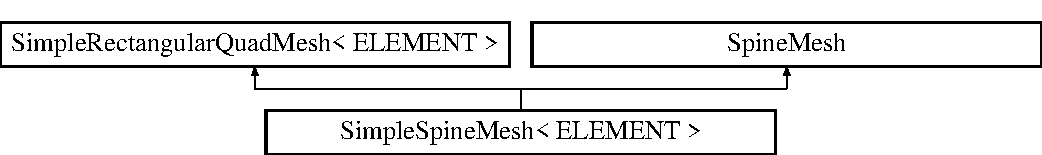
\includegraphics[height=2.000000cm]{classSimpleSpineMesh}
\end{center}
\end{figure}
\subsection*{Public Types}
\begin{DoxyCompactItemize}
\item 
typedef double($\ast$ \hyperlink{classSimpleSpineMesh_a671d96f0143dfeb7aaba8af56c0c0620}{Height\+Fct\+Pt}) (const double \&x)
\begin{DoxyCompactList}\small\item\em Function pointer to function, h(x), that may be used to specify the \char`\"{}height\char`\"{} of the domain, by assigning the function values to the spine heights. \end{DoxyCompactList}\end{DoxyCompactItemize}
\subsection*{Public Member Functions}
\begin{DoxyCompactItemize}
\item 
\hyperlink{classSimpleSpineMesh_a69815e3a950e6e5ede2f85004796dadb}{Simple\+Spine\+Mesh} (const unsigned \&nx, const unsigned \&ny, const double \&lx, const double \&h, Geom\+Object $\ast$substrate\+\_\+pt, Time\+Stepper $\ast$time\+\_\+stepper\+\_\+pt=\&Mesh\+::\+Default\+\_\+\+Time\+Stepper)
\begin{DoxyCompactList}\small\item\em Constructor\+: Pass number of elements in x-\/direction, number of elements in y-\/direction, length in x direction, initial height of mesh, and pointer to timestepper (defaults to Steady timestepper) \end{DoxyCompactList}\item 
\hyperlink{classSimpleSpineMesh_a671d96f0143dfeb7aaba8af56c0c0620}{Height\+Fct\+Pt} \& \hyperlink{classSimpleSpineMesh_af84290225b4aea3fd6ba27ad979059a0}{height\+\_\+fct\+\_\+pt} ()
\begin{DoxyCompactList}\small\item\em Access function\+: Pointer to height function. \end{DoxyCompactList}\item 
double \hyperlink{classSimpleSpineMesh_a99398fc7ef50db36d30f6c1d01aa3758}{height\+\_\+fct} (const double \&x)
\begin{DoxyCompactList}\small\item\em Height function -- this is called by \hyperlink{classSimpleSpineMesh_a2248fb8df448b0a02377a0cfb6f57851}{update\+\_\+spine\+\_\+heights()} when spine heights are assigned. \end{DoxyCompactList}\item 
void \hyperlink{classSimpleSpineMesh_a2248fb8df448b0a02377a0cfb6f57851}{update\+\_\+spine\+\_\+heights} ()
\begin{DoxyCompactList}\small\item\em Update the spine heights according to the function specified by \hyperlink{classSimpleSpineMesh_af84290225b4aea3fd6ba27ad979059a0}{height\+\_\+fct\+\_\+pt()}. \end{DoxyCompactList}\item 
virtual void \hyperlink{classSimpleSpineMesh_a4735e047eab146cafc3090f829373ef2}{spine\+\_\+node\+\_\+update} (Spine\+Node $\ast$spine\+\_\+node\+\_\+pt)
\begin{DoxyCompactList}\small\item\em General node update function implements pure virtual function defined in Spine\+Mesh base class and performs specific node update actions\+: Nodes are located along vertical \char`\"{}spines\char`\"{} that emanate from the \char`\"{}substrate\char`\"{} (the lower wall) specified by a Geom\+Object. \end{DoxyCompactList}\end{DoxyCompactItemize}
\subsection*{Private Attributes}
\begin{DoxyCompactItemize}
\item 
double \hyperlink{classSimpleSpineMesh_a7a6d3f655da48ed9d18f6ca8e29f6576}{Default\+\_\+height}
\begin{DoxyCompactList}\small\item\em Default height. \end{DoxyCompactList}\item 
\hyperlink{classSimpleSpineMesh_a671d96f0143dfeb7aaba8af56c0c0620}{Height\+Fct\+Pt} \hyperlink{classSimpleSpineMesh_ac0509d0d0868d37ef87834b39d2a084b}{Height\+\_\+fct\+\_\+pt}
\begin{DoxyCompactList}\small\item\em Pointer to height function. \end{DoxyCompactList}\item 
Geom\+Object $\ast$ \hyperlink{classSimpleSpineMesh_a9031e27d5855e029312d356f6a38da76}{Substrate\+\_\+pt}
\begin{DoxyCompactList}\small\item\em Pointer to Geom\+Object that specifies the \char`\"{}substrate\char`\"{} (the lower wall) \end{DoxyCompactList}\end{DoxyCompactItemize}


\subsection{Detailed Description}
\subsubsection*{template$<$class E\+L\+E\+M\+E\+NT$>$\newline
class Simple\+Spine\+Mesh$<$ E\+L\+E\+M\+E\+N\+T $>$}

Simple spine mesh class derived from standard 2D mesh. Vertical lines of nodes are located on spines. 

Definition at line 93 of file simple\+\_\+spine\+\_\+channel.\+cc.



\subsection{Member Typedef Documentation}
\mbox{\Hypertarget{classSimpleSpineMesh_a671d96f0143dfeb7aaba8af56c0c0620}\label{classSimpleSpineMesh_a671d96f0143dfeb7aaba8af56c0c0620}} 
\index{Simple\+Spine\+Mesh@{Simple\+Spine\+Mesh}!Height\+Fct\+Pt@{Height\+Fct\+Pt}}
\index{Height\+Fct\+Pt@{Height\+Fct\+Pt}!Simple\+Spine\+Mesh@{Simple\+Spine\+Mesh}}
\subsubsection{\texorpdfstring{Height\+Fct\+Pt}{HeightFctPt}}
{\footnotesize\ttfamily template$<$class E\+L\+E\+M\+E\+NT$>$ \\
typedef double($\ast$ \hyperlink{classSimpleSpineMesh}{Simple\+Spine\+Mesh}$<$ E\+L\+E\+M\+E\+NT $>$\+::Height\+Fct\+Pt) (const double \&x)}



Function pointer to function, h(x), that may be used to specify the \char`\"{}height\char`\"{} of the domain, by assigning the function values to the spine heights. 



Definition at line 114 of file simple\+\_\+spine\+\_\+channel.\+cc.



\subsection{Constructor \& Destructor Documentation}
\mbox{\Hypertarget{classSimpleSpineMesh_a69815e3a950e6e5ede2f85004796dadb}\label{classSimpleSpineMesh_a69815e3a950e6e5ede2f85004796dadb}} 
\index{Simple\+Spine\+Mesh@{Simple\+Spine\+Mesh}!Simple\+Spine\+Mesh@{Simple\+Spine\+Mesh}}
\index{Simple\+Spine\+Mesh@{Simple\+Spine\+Mesh}!Simple\+Spine\+Mesh@{Simple\+Spine\+Mesh}}
\subsubsection{\texorpdfstring{Simple\+Spine\+Mesh()}{SimpleSpineMesh()}}
{\footnotesize\ttfamily template$<$class E\+L\+E\+M\+E\+NT $>$ \\
\hyperlink{classSimpleSpineMesh}{Simple\+Spine\+Mesh}$<$ E\+L\+E\+M\+E\+NT $>$\+::\hyperlink{classSimpleSpineMesh}{Simple\+Spine\+Mesh} (\begin{DoxyParamCaption}\item[{const unsigned \&}]{nx,  }\item[{const unsigned \&}]{ny,  }\item[{const double \&}]{lx,  }\item[{const double \&}]{h,  }\item[{Geom\+Object $\ast$}]{substrate\+\_\+pt,  }\item[{Time\+Stepper $\ast$}]{time\+\_\+stepper\+\_\+pt = {\ttfamily \&Mesh\+:\+:Default\+\_\+TimeStepper} }\end{DoxyParamCaption})}



Constructor\+: Pass number of elements in x-\/direction, number of elements in y-\/direction, length in x direction, initial height of mesh, and pointer to timestepper (defaults to Steady timestepper) 

Constructor for spine 2D mesh\+: Pass number of elements in x-\/direction, number of elements in y-\/direction, axial length and height of layer, pointer to geometric object that specifies the substrate (the lower wall) and pointer to timestepper (defaults to Static timestepper).

The mesh contains a layer of spine-\/ified fluid elements (of type E\+L\+E\+M\+E\+NT; e.\+g Spine\+Element$<$Q\+Crouzeix\+Raviart\+Element$<$2$>$) 

Definition at line 210 of file simple\+\_\+spine\+\_\+channel.\+cc.



References Simple\+Spine\+Mesh$<$ E\+L\+E\+M\+E\+N\+T $>$\+::\+Substrate\+\_\+pt.



\subsection{Member Function Documentation}
\mbox{\Hypertarget{classSimpleSpineMesh_a99398fc7ef50db36d30f6c1d01aa3758}\label{classSimpleSpineMesh_a99398fc7ef50db36d30f6c1d01aa3758}} 
\index{Simple\+Spine\+Mesh@{Simple\+Spine\+Mesh}!height\+\_\+fct@{height\+\_\+fct}}
\index{height\+\_\+fct@{height\+\_\+fct}!Simple\+Spine\+Mesh@{Simple\+Spine\+Mesh}}
\subsubsection{\texorpdfstring{height\+\_\+fct()}{height\_fct()}}
{\footnotesize\ttfamily template$<$class E\+L\+E\+M\+E\+NT$>$ \\
double \hyperlink{classSimpleSpineMesh}{Simple\+Spine\+Mesh}$<$ E\+L\+E\+M\+E\+NT $>$\+::height\+\_\+fct (\begin{DoxyParamCaption}\item[{const double \&}]{x }\end{DoxyParamCaption})\hspace{0.3cm}{\ttfamily [inline]}}



Height function -- this is called by \hyperlink{classSimpleSpineMesh_a2248fb8df448b0a02377a0cfb6f57851}{update\+\_\+spine\+\_\+heights()} when spine heights are assigned. 



Definition at line 125 of file simple\+\_\+spine\+\_\+channel.\+cc.

\mbox{\Hypertarget{classSimpleSpineMesh_af84290225b4aea3fd6ba27ad979059a0}\label{classSimpleSpineMesh_af84290225b4aea3fd6ba27ad979059a0}} 
\index{Simple\+Spine\+Mesh@{Simple\+Spine\+Mesh}!height\+\_\+fct\+\_\+pt@{height\+\_\+fct\+\_\+pt}}
\index{height\+\_\+fct\+\_\+pt@{height\+\_\+fct\+\_\+pt}!Simple\+Spine\+Mesh@{Simple\+Spine\+Mesh}}
\subsubsection{\texorpdfstring{height\+\_\+fct\+\_\+pt()}{height\_fct\_pt()}}
{\footnotesize\ttfamily template$<$class E\+L\+E\+M\+E\+NT$>$ \\
\hyperlink{classSimpleSpineMesh_a671d96f0143dfeb7aaba8af56c0c0620}{Height\+Fct\+Pt}\& \hyperlink{classSimpleSpineMesh}{Simple\+Spine\+Mesh}$<$ E\+L\+E\+M\+E\+NT $>$\+::height\+\_\+fct\+\_\+pt (\begin{DoxyParamCaption}{ }\end{DoxyParamCaption})\hspace{0.3cm}{\ttfamily [inline]}}



Access function\+: Pointer to height function. 



Definition at line 117 of file simple\+\_\+spine\+\_\+channel.\+cc.



Referenced by Channel\+Spine\+Flow\+Problem$<$ E\+L\+E\+M\+E\+N\+T $>$\+::\+Channel\+Spine\+Flow\+Problem().

\mbox{\Hypertarget{classSimpleSpineMesh_a4735e047eab146cafc3090f829373ef2}\label{classSimpleSpineMesh_a4735e047eab146cafc3090f829373ef2}} 
\index{Simple\+Spine\+Mesh@{Simple\+Spine\+Mesh}!spine\+\_\+node\+\_\+update@{spine\+\_\+node\+\_\+update}}
\index{spine\+\_\+node\+\_\+update@{spine\+\_\+node\+\_\+update}!Simple\+Spine\+Mesh@{Simple\+Spine\+Mesh}}
\subsubsection{\texorpdfstring{spine\+\_\+node\+\_\+update()}{spine\_node\_update()}}
{\footnotesize\ttfamily template$<$class E\+L\+E\+M\+E\+NT$>$ \\
virtual void \hyperlink{classSimpleSpineMesh}{Simple\+Spine\+Mesh}$<$ E\+L\+E\+M\+E\+NT $>$\+::spine\+\_\+node\+\_\+update (\begin{DoxyParamCaption}\item[{Spine\+Node $\ast$}]{spine\+\_\+node\+\_\+pt }\end{DoxyParamCaption})\hspace{0.3cm}{\ttfamily [inline]}, {\ttfamily [virtual]}}



General node update function implements pure virtual function defined in Spine\+Mesh base class and performs specific node update actions\+: Nodes are located along vertical \char`\"{}spines\char`\"{} that emanate from the \char`\"{}substrate\char`\"{} (the lower wall) specified by a Geom\+Object. 



Definition at line 161 of file simple\+\_\+spine\+\_\+channel.\+cc.

\mbox{\Hypertarget{classSimpleSpineMesh_a2248fb8df448b0a02377a0cfb6f57851}\label{classSimpleSpineMesh_a2248fb8df448b0a02377a0cfb6f57851}} 
\index{Simple\+Spine\+Mesh@{Simple\+Spine\+Mesh}!update\+\_\+spine\+\_\+heights@{update\+\_\+spine\+\_\+heights}}
\index{update\+\_\+spine\+\_\+heights@{update\+\_\+spine\+\_\+heights}!Simple\+Spine\+Mesh@{Simple\+Spine\+Mesh}}
\subsubsection{\texorpdfstring{update\+\_\+spine\+\_\+heights()}{update\_spine\_heights()}}
{\footnotesize\ttfamily template$<$class E\+L\+E\+M\+E\+NT$>$ \\
void \hyperlink{classSimpleSpineMesh}{Simple\+Spine\+Mesh}$<$ E\+L\+E\+M\+E\+NT $>$\+::update\+\_\+spine\+\_\+heights (\begin{DoxyParamCaption}{ }\end{DoxyParamCaption})\hspace{0.3cm}{\ttfamily [inline]}}



Update the spine heights according to the function specified by \hyperlink{classSimpleSpineMesh_af84290225b4aea3fd6ba27ad979059a0}{height\+\_\+fct\+\_\+pt()}. 



Definition at line 141 of file simple\+\_\+spine\+\_\+channel.\+cc.



\subsection{Member Data Documentation}
\mbox{\Hypertarget{classSimpleSpineMesh_a7a6d3f655da48ed9d18f6ca8e29f6576}\label{classSimpleSpineMesh_a7a6d3f655da48ed9d18f6ca8e29f6576}} 
\index{Simple\+Spine\+Mesh@{Simple\+Spine\+Mesh}!Default\+\_\+height@{Default\+\_\+height}}
\index{Default\+\_\+height@{Default\+\_\+height}!Simple\+Spine\+Mesh@{Simple\+Spine\+Mesh}}
\subsubsection{\texorpdfstring{Default\+\_\+height}{Default\_height}}
{\footnotesize\ttfamily template$<$class E\+L\+E\+M\+E\+NT$>$ \\
double \hyperlink{classSimpleSpineMesh}{Simple\+Spine\+Mesh}$<$ E\+L\+E\+M\+E\+NT $>$\+::Default\+\_\+height\hspace{0.3cm}{\ttfamily [private]}}



Default height. 



Definition at line 188 of file simple\+\_\+spine\+\_\+channel.\+cc.

\mbox{\Hypertarget{classSimpleSpineMesh_ac0509d0d0868d37ef87834b39d2a084b}\label{classSimpleSpineMesh_ac0509d0d0868d37ef87834b39d2a084b}} 
\index{Simple\+Spine\+Mesh@{Simple\+Spine\+Mesh}!Height\+\_\+fct\+\_\+pt@{Height\+\_\+fct\+\_\+pt}}
\index{Height\+\_\+fct\+\_\+pt@{Height\+\_\+fct\+\_\+pt}!Simple\+Spine\+Mesh@{Simple\+Spine\+Mesh}}
\subsubsection{\texorpdfstring{Height\+\_\+fct\+\_\+pt}{Height\_fct\_pt}}
{\footnotesize\ttfamily template$<$class E\+L\+E\+M\+E\+NT$>$ \\
\hyperlink{classSimpleSpineMesh_a671d96f0143dfeb7aaba8af56c0c0620}{Height\+Fct\+Pt} \hyperlink{classSimpleSpineMesh}{Simple\+Spine\+Mesh}$<$ E\+L\+E\+M\+E\+NT $>$\+::Height\+\_\+fct\+\_\+pt\hspace{0.3cm}{\ttfamily [private]}}



Pointer to height function. 



Definition at line 191 of file simple\+\_\+spine\+\_\+channel.\+cc.

\mbox{\Hypertarget{classSimpleSpineMesh_a9031e27d5855e029312d356f6a38da76}\label{classSimpleSpineMesh_a9031e27d5855e029312d356f6a38da76}} 
\index{Simple\+Spine\+Mesh@{Simple\+Spine\+Mesh}!Substrate\+\_\+pt@{Substrate\+\_\+pt}}
\index{Substrate\+\_\+pt@{Substrate\+\_\+pt}!Simple\+Spine\+Mesh@{Simple\+Spine\+Mesh}}
\subsubsection{\texorpdfstring{Substrate\+\_\+pt}{Substrate\_pt}}
{\footnotesize\ttfamily template$<$class E\+L\+E\+M\+E\+NT$>$ \\
Geom\+Object$\ast$ \hyperlink{classSimpleSpineMesh}{Simple\+Spine\+Mesh}$<$ E\+L\+E\+M\+E\+NT $>$\+::Substrate\+\_\+pt\hspace{0.3cm}{\ttfamily [private]}}



Pointer to Geom\+Object that specifies the \char`\"{}substrate\char`\"{} (the lower wall) 



Definition at line 194 of file simple\+\_\+spine\+\_\+channel.\+cc.



Referenced by Simple\+Spine\+Mesh$<$ E\+L\+E\+M\+E\+N\+T $>$\+::\+Simple\+Spine\+Mesh().



The documentation for this class was generated from the following file\+:\begin{DoxyCompactItemize}
\item 
\hyperlink{simple__spine__channel_8cc}{simple\+\_\+spine\+\_\+channel.\+cc}\end{DoxyCompactItemize}

\hypertarget{classSinusoidalWall}{}\section{Sinusoidal\+Wall Class Reference}
\label{classSinusoidalWall}\index{Sinusoidal\+Wall@{Sinusoidal\+Wall}}
Inheritance diagram for Sinusoidal\+Wall\+:\begin{figure}[H]
\begin{center}
\leavevmode
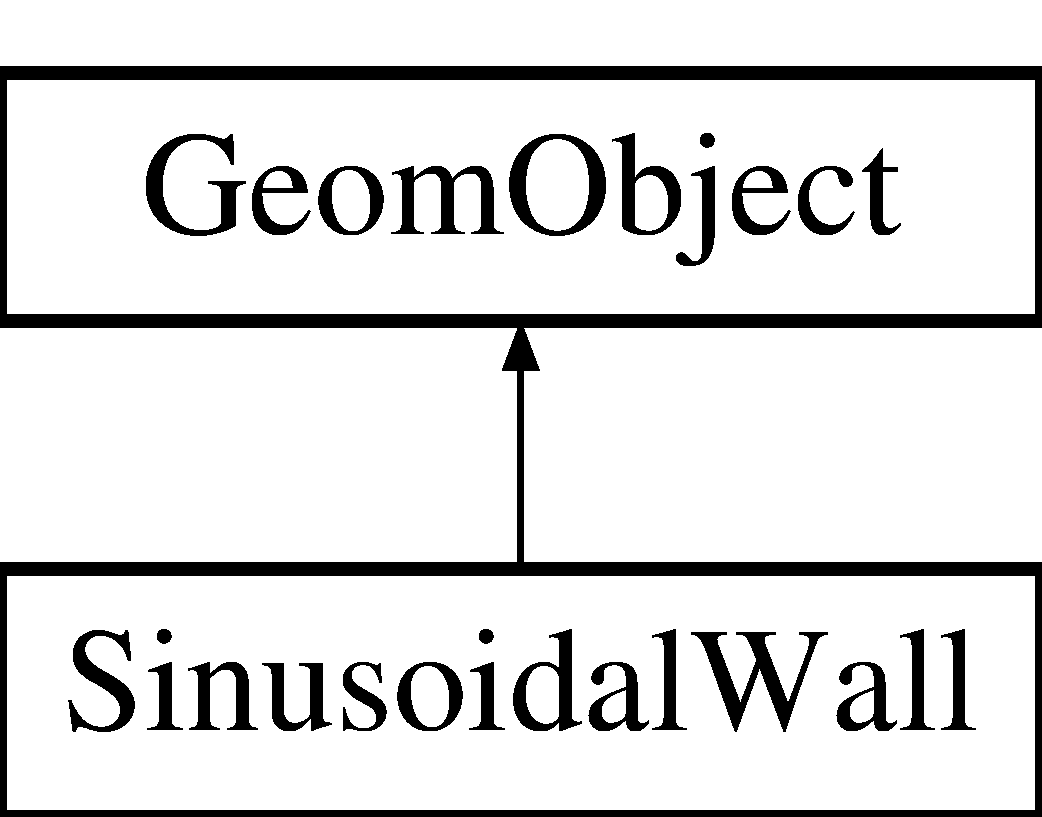
\includegraphics[height=2.000000cm]{classSinusoidalWall}
\end{center}
\end{figure}
\subsection*{Public Member Functions}
\begin{DoxyCompactItemize}
\item 
\hyperlink{classSinusoidalWall_a6179a8823d039fc3b090db1cfce30a36}{Sinusoidal\+Wall} (const double \&\hyperlink{classSinusoidalWall_a78861ab97b81bc78e05c3ec260c6479d}{height}, const double \&\hyperlink{classSinusoidalWall_a654a7ccf081040971442d8534f1e6807}{amplitude}, const double \&zeta\+\_\+min, const double \&zeta\+\_\+max)
\begin{DoxyCompactList}\small\item\em Constructor\+: Pass height, amplitude, zeta min and zeta max (all are pinned by default) \end{DoxyCompactList}\item 
\hyperlink{classSinusoidalWall_ac437fb52cca5a1b467f6f87ecc2c75aa}{Sinusoidal\+Wall} (const Vector$<$ Data $\ast$$>$ \&\hyperlink{classSinusoidalWall_ab9dc7c9e02dac3171c378cea6949f544}{geom\+\_\+data\+\_\+pt})
\begin{DoxyCompactList}\small\item\em Constructor\+: One item of geometric data, containing four values\+: \end{DoxyCompactList}\item 
\hyperlink{classSinusoidalWall_a7e5c29a951c707cb87e168ed943a7956}{$\sim$\+Sinusoidal\+Wall} ()
\begin{DoxyCompactList}\small\item\em Destructor\+: Clean up if necessary. \end{DoxyCompactList}\item 
double \& \hyperlink{classSinusoidalWall_a78861ab97b81bc78e05c3ec260c6479d}{height} ()
\begin{DoxyCompactList}\small\item\em Access function for horizontal half axis. \end{DoxyCompactList}\item 
double \& \hyperlink{classSinusoidalWall_a654a7ccf081040971442d8534f1e6807}{amplitude} ()
\begin{DoxyCompactList}\small\item\em Access function for vertical half axis. \end{DoxyCompactList}\item 
void \hyperlink{classSinusoidalWall_a8a1ce17bdb30f20894e1d85668877502}{position} (const Vector$<$ double $>$ \&zeta, Vector$<$ double $>$ \&r) const
\begin{DoxyCompactList}\small\item\em Position vector at Lagrangian coordinate zeta. \end{DoxyCompactList}\item 
void \hyperlink{classSinusoidalWall_afe74256b6e259c0c939a839db13a40cd}{position} (const unsigned \&t, const Vector$<$ double $>$ \&zeta, Vector$<$ double $>$ \&r) const
\begin{DoxyCompactList}\small\item\em Parametrised position on object\+: r(zeta). Evaluated at previous timestep. t=0\+: current time; t$>$0\+: previous timestep. \end{DoxyCompactList}\item 
virtual void \hyperlink{classSinusoidalWall_a3ab79b227fd0bae3694737099c519346}{dposition} (const Vector$<$ double $>$ \&zeta, Dense\+Matrix$<$ double $>$ \&drdzeta) const
\begin{DoxyCompactList}\small\item\em Derivative of position Vector w.\+r.\+t. to coordinates\+: $ \frac{dR_i}{d \zeta_\alpha}$ = drdzeta(alpha,i). Evaluated at current time. \end{DoxyCompactList}\item 
virtual void \hyperlink{classSinusoidalWall_a96bda32ccbca0aa16a5d7e43ed2376e9}{d2position} (const Vector$<$ double $>$ \&zeta, Rank\+Three\+Tensor$<$ double $>$ \&ddrdzeta) const
\begin{DoxyCompactList}\small\item\em 2nd derivative of position Vector w.\+r.\+t. to coordinates\+: $ \frac{d^2R_i}{d \zeta_\alpha d \zeta_\beta}$ = ddrdzeta(alpha,beta,i). Evaluated at current time. \end{DoxyCompactList}\item 
virtual void \hyperlink{classSinusoidalWall_aa0910636dfb4aa6d14e1a6bd012da573}{d2position} (const Vector$<$ double $>$ \&zeta, Vector$<$ double $>$ \&r, Dense\+Matrix$<$ double $>$ \&drdzeta, Rank\+Three\+Tensor$<$ double $>$ \&ddrdzeta) const
\begin{DoxyCompactList}\small\item\em Posn Vector and its 1st \& 2nd derivatives w.\+r.\+t. to coordinates\+: $ \frac{dR_i}{d \zeta_\alpha}$ = drdzeta(alpha,i). $ \frac{d^2R_i}{d \zeta_\alpha d \zeta_\beta}$ = ddrdzeta(alpha,beta,i). Evaluated at current time. \end{DoxyCompactList}\item 
unsigned \hyperlink{classSinusoidalWall_ada343bc36f0d4dd1a0b79da62d10c33d}{ngeom\+\_\+data} () const
\begin{DoxyCompactList}\small\item\em How many items of Data does the shape of the object depend on? \end{DoxyCompactList}\item 
Data $\ast$ \hyperlink{classSinusoidalWall_ab9dc7c9e02dac3171c378cea6949f544}{geom\+\_\+data\+\_\+pt} (const unsigned \&j)
\begin{DoxyCompactList}\small\item\em Return pointer to the j-\/th Data item that the object\textquotesingle{}s shape depends on. \end{DoxyCompactList}\end{DoxyCompactItemize}
\subsection*{Private Attributes}
\begin{DoxyCompactItemize}
\item 
Vector$<$ Data $\ast$ $>$ \hyperlink{classSinusoidalWall_a1d8226424f058dff0234e65a6e288a39}{Geom\+\_\+data\+\_\+pt}
\begin{DoxyCompactList}\small\item\em Vector of pointers to Data items that affects the object\textquotesingle{}s shape. \end{DoxyCompactList}\item 
bool \hyperlink{classSinusoidalWall_ad89b819030680f489135376a8abc9f05}{Must\+\_\+clean\+\_\+up}
\begin{DoxyCompactList}\small\item\em Do I need to clean up? \end{DoxyCompactList}\end{DoxyCompactItemize}


\subsection{Detailed Description}
Geometric object representing a sinusoidal wall, parametrised by \[ x = \zeta \] \[ y = H + A \sin\left(\frac{2\pi \left(\zeta-\zeta_{\mbox{min}}\right)} {\zeta_{\mbox{max}}-\zeta_{\mbox{min}}} \right)\] 

Definition at line 76 of file spine\+\_\+channel.\+cc.



\subsection{Constructor \& Destructor Documentation}
\mbox{\Hypertarget{classSinusoidalWall_a6179a8823d039fc3b090db1cfce30a36}\label{classSinusoidalWall_a6179a8823d039fc3b090db1cfce30a36}} 
\index{Sinusoidal\+Wall@{Sinusoidal\+Wall}!Sinusoidal\+Wall@{Sinusoidal\+Wall}}
\index{Sinusoidal\+Wall@{Sinusoidal\+Wall}!Sinusoidal\+Wall@{Sinusoidal\+Wall}}
\subsubsection{\texorpdfstring{Sinusoidal\+Wall()}{SinusoidalWall()}\hspace{0.1cm}{\footnotesize\ttfamily [1/2]}}
{\footnotesize\ttfamily Sinusoidal\+Wall\+::\+Sinusoidal\+Wall (\begin{DoxyParamCaption}\item[{const double \&}]{height,  }\item[{const double \&}]{amplitude,  }\item[{const double \&}]{zeta\+\_\+min,  }\item[{const double \&}]{zeta\+\_\+max }\end{DoxyParamCaption})\hspace{0.3cm}{\ttfamily [inline]}}



Constructor\+: Pass height, amplitude, zeta min and zeta max (all are pinned by default) 



Definition at line 83 of file spine\+\_\+channel.\+cc.

\mbox{\Hypertarget{classSinusoidalWall_ac437fb52cca5a1b467f6f87ecc2c75aa}\label{classSinusoidalWall_ac437fb52cca5a1b467f6f87ecc2c75aa}} 
\index{Sinusoidal\+Wall@{Sinusoidal\+Wall}!Sinusoidal\+Wall@{Sinusoidal\+Wall}}
\index{Sinusoidal\+Wall@{Sinusoidal\+Wall}!Sinusoidal\+Wall@{Sinusoidal\+Wall}}
\subsubsection{\texorpdfstring{Sinusoidal\+Wall()}{SinusoidalWall()}\hspace{0.1cm}{\footnotesize\ttfamily [2/2]}}
{\footnotesize\ttfamily Sinusoidal\+Wall\+::\+Sinusoidal\+Wall (\begin{DoxyParamCaption}\item[{const Vector$<$ Data $\ast$$>$ \&}]{geom\+\_\+data\+\_\+pt }\end{DoxyParamCaption})\hspace{0.3cm}{\ttfamily [inline]}}



Constructor\+: One item of geometric data, containing four values\+: 


\begin{DoxyCode}
\hyperlink{classSinusoidalWall_a1d8226424f058dff0234e65a6e288a39}{Geom\_data\_pt}[0]->value(0) = \hyperlink{classSinusoidalWall_a78861ab97b81bc78e05c3ec260c6479d}{height}
\hyperlink{classSinusoidalWall_a1d8226424f058dff0234e65a6e288a39}{Geom\_data\_pt}[0]->value(1) = \hyperlink{classSinusoidalWall_a654a7ccf081040971442d8534f1e6807}{amplitude}
\hyperlink{classSinusoidalWall_a1d8226424f058dff0234e65a6e288a39}{Geom\_data\_pt}[0]->value(2) = zeta\_min
\hyperlink{classSinusoidalWall_a1d8226424f058dff0234e65a6e288a39}{Geom\_data\_pt}[0]->value(3) = zeta\_max
\end{DoxyCode}
 

Definition at line 115 of file spine\+\_\+channel.\+cc.

\mbox{\Hypertarget{classSinusoidalWall_a7e5c29a951c707cb87e168ed943a7956}\label{classSinusoidalWall_a7e5c29a951c707cb87e168ed943a7956}} 
\index{Sinusoidal\+Wall@{Sinusoidal\+Wall}!````~Sinusoidal\+Wall@{$\sim$\+Sinusoidal\+Wall}}
\index{````~Sinusoidal\+Wall@{$\sim$\+Sinusoidal\+Wall}!Sinusoidal\+Wall@{Sinusoidal\+Wall}}
\subsubsection{\texorpdfstring{$\sim$\+Sinusoidal\+Wall()}{~SinusoidalWall()}}
{\footnotesize\ttfamily Sinusoidal\+Wall\+::$\sim$\+Sinusoidal\+Wall (\begin{DoxyParamCaption}{ }\end{DoxyParamCaption})\hspace{0.3cm}{\ttfamily [inline]}}



Destructor\+: Clean up if necessary. 



Definition at line 144 of file spine\+\_\+channel.\+cc.



\subsection{Member Function Documentation}
\mbox{\Hypertarget{classSinusoidalWall_a654a7ccf081040971442d8534f1e6807}\label{classSinusoidalWall_a654a7ccf081040971442d8534f1e6807}} 
\index{Sinusoidal\+Wall@{Sinusoidal\+Wall}!amplitude@{amplitude}}
\index{amplitude@{amplitude}!Sinusoidal\+Wall@{Sinusoidal\+Wall}}
\subsubsection{\texorpdfstring{amplitude()}{amplitude()}}
{\footnotesize\ttfamily double\& Sinusoidal\+Wall\+::amplitude (\begin{DoxyParamCaption}{ }\end{DoxyParamCaption})\hspace{0.3cm}{\ttfamily [inline]}}



Access function for vertical half axis. 



Definition at line 158 of file spine\+\_\+channel.\+cc.

\mbox{\Hypertarget{classSinusoidalWall_a96bda32ccbca0aa16a5d7e43ed2376e9}\label{classSinusoidalWall_a96bda32ccbca0aa16a5d7e43ed2376e9}} 
\index{Sinusoidal\+Wall@{Sinusoidal\+Wall}!d2position@{d2position}}
\index{d2position@{d2position}!Sinusoidal\+Wall@{Sinusoidal\+Wall}}
\subsubsection{\texorpdfstring{d2position()}{d2position()}\hspace{0.1cm}{\footnotesize\ttfamily [1/2]}}
{\footnotesize\ttfamily virtual void Sinusoidal\+Wall\+::d2position (\begin{DoxyParamCaption}\item[{const Vector$<$ double $>$ \&}]{zeta,  }\item[{Rank\+Three\+Tensor$<$ double $>$ \&}]{ddrdzeta }\end{DoxyParamCaption}) const\hspace{0.3cm}{\ttfamily [inline]}, {\ttfamily [virtual]}}



2nd derivative of position Vector w.\+r.\+t. to coordinates\+: $ \frac{d^2R_i}{d \zeta_\alpha d \zeta_\beta}$ = ddrdzeta(alpha,beta,i). Evaluated at current time. 



Definition at line 241 of file spine\+\_\+channel.\+cc.



References Global\+\_\+\+Physical\+\_\+\+Variables\+::A.

\mbox{\Hypertarget{classSinusoidalWall_aa0910636dfb4aa6d14e1a6bd012da573}\label{classSinusoidalWall_aa0910636dfb4aa6d14e1a6bd012da573}} 
\index{Sinusoidal\+Wall@{Sinusoidal\+Wall}!d2position@{d2position}}
\index{d2position@{d2position}!Sinusoidal\+Wall@{Sinusoidal\+Wall}}
\subsubsection{\texorpdfstring{d2position()}{d2position()}\hspace{0.1cm}{\footnotesize\ttfamily [2/2]}}
{\footnotesize\ttfamily virtual void Sinusoidal\+Wall\+::d2position (\begin{DoxyParamCaption}\item[{const Vector$<$ double $>$ \&}]{zeta,  }\item[{Vector$<$ double $>$ \&}]{r,  }\item[{Dense\+Matrix$<$ double $>$ \&}]{drdzeta,  }\item[{Rank\+Three\+Tensor$<$ double $>$ \&}]{ddrdzeta }\end{DoxyParamCaption}) const\hspace{0.3cm}{\ttfamily [inline]}, {\ttfamily [virtual]}}



Posn Vector and its 1st \& 2nd derivatives w.\+r.\+t. to coordinates\+: $ \frac{dR_i}{d \zeta_\alpha}$ = drdzeta(alpha,i). $ \frac{d^2R_i}{d \zeta_\alpha d \zeta_\beta}$ = ddrdzeta(alpha,beta,i). Evaluated at current time. 



Definition at line 262 of file spine\+\_\+channel.\+cc.



References Global\+\_\+\+Physical\+\_\+\+Variables\+::A, and Global\+\_\+\+Physical\+\_\+\+Variables\+::H.

\mbox{\Hypertarget{classSinusoidalWall_a3ab79b227fd0bae3694737099c519346}\label{classSinusoidalWall_a3ab79b227fd0bae3694737099c519346}} 
\index{Sinusoidal\+Wall@{Sinusoidal\+Wall}!dposition@{dposition}}
\index{dposition@{dposition}!Sinusoidal\+Wall@{Sinusoidal\+Wall}}
\subsubsection{\texorpdfstring{dposition()}{dposition()}}
{\footnotesize\ttfamily virtual void Sinusoidal\+Wall\+::dposition (\begin{DoxyParamCaption}\item[{const Vector$<$ double $>$ \&}]{zeta,  }\item[{Dense\+Matrix$<$ double $>$ \&}]{drdzeta }\end{DoxyParamCaption}) const\hspace{0.3cm}{\ttfamily [inline]}, {\ttfamily [virtual]}}



Derivative of position Vector w.\+r.\+t. to coordinates\+: $ \frac{dR_i}{d \zeta_\alpha}$ = drdzeta(alpha,i). Evaluated at current time. 



Definition at line 222 of file spine\+\_\+channel.\+cc.



References Global\+\_\+\+Physical\+\_\+\+Variables\+::A.

\mbox{\Hypertarget{classSinusoidalWall_ab9dc7c9e02dac3171c378cea6949f544}\label{classSinusoidalWall_ab9dc7c9e02dac3171c378cea6949f544}} 
\index{Sinusoidal\+Wall@{Sinusoidal\+Wall}!geom\+\_\+data\+\_\+pt@{geom\+\_\+data\+\_\+pt}}
\index{geom\+\_\+data\+\_\+pt@{geom\+\_\+data\+\_\+pt}!Sinusoidal\+Wall@{Sinusoidal\+Wall}}
\subsubsection{\texorpdfstring{geom\+\_\+data\+\_\+pt()}{geom\_data\_pt()}}
{\footnotesize\ttfamily Data$\ast$ Sinusoidal\+Wall\+::geom\+\_\+data\+\_\+pt (\begin{DoxyParamCaption}\item[{const unsigned \&}]{j }\end{DoxyParamCaption})\hspace{0.3cm}{\ttfamily [inline]}}



Return pointer to the j-\/th Data item that the object\textquotesingle{}s shape depends on. 



Definition at line 293 of file spine\+\_\+channel.\+cc.

\mbox{\Hypertarget{classSinusoidalWall_a78861ab97b81bc78e05c3ec260c6479d}\label{classSinusoidalWall_a78861ab97b81bc78e05c3ec260c6479d}} 
\index{Sinusoidal\+Wall@{Sinusoidal\+Wall}!height@{height}}
\index{height@{height}!Sinusoidal\+Wall@{Sinusoidal\+Wall}}
\subsubsection{\texorpdfstring{height()}{height()}}
{\footnotesize\ttfamily double\& Sinusoidal\+Wall\+::height (\begin{DoxyParamCaption}{ }\end{DoxyParamCaption})\hspace{0.3cm}{\ttfamily [inline]}}



Access function for horizontal half axis. 



Definition at line 155 of file spine\+\_\+channel.\+cc.

\mbox{\Hypertarget{classSinusoidalWall_ada343bc36f0d4dd1a0b79da62d10c33d}\label{classSinusoidalWall_ada343bc36f0d4dd1a0b79da62d10c33d}} 
\index{Sinusoidal\+Wall@{Sinusoidal\+Wall}!ngeom\+\_\+data@{ngeom\+\_\+data}}
\index{ngeom\+\_\+data@{ngeom\+\_\+data}!Sinusoidal\+Wall@{Sinusoidal\+Wall}}
\subsubsection{\texorpdfstring{ngeom\+\_\+data()}{ngeom\_data()}}
{\footnotesize\ttfamily unsigned Sinusoidal\+Wall\+::ngeom\+\_\+data (\begin{DoxyParamCaption}{ }\end{DoxyParamCaption}) const\hspace{0.3cm}{\ttfamily [inline]}}



How many items of Data does the shape of the object depend on? 



Definition at line 289 of file spine\+\_\+channel.\+cc.

\mbox{\Hypertarget{classSinusoidalWall_a8a1ce17bdb30f20894e1d85668877502}\label{classSinusoidalWall_a8a1ce17bdb30f20894e1d85668877502}} 
\index{Sinusoidal\+Wall@{Sinusoidal\+Wall}!position@{position}}
\index{position@{position}!Sinusoidal\+Wall@{Sinusoidal\+Wall}}
\subsubsection{\texorpdfstring{position()}{position()}\hspace{0.1cm}{\footnotesize\ttfamily [1/2]}}
{\footnotesize\ttfamily void Sinusoidal\+Wall\+::position (\begin{DoxyParamCaption}\item[{const Vector$<$ double $>$ \&}]{zeta,  }\item[{Vector$<$ double $>$ \&}]{r }\end{DoxyParamCaption}) const\hspace{0.3cm}{\ttfamily [inline]}}



Position vector at Lagrangian coordinate zeta. 



Definition at line 162 of file spine\+\_\+channel.\+cc.



References Global\+\_\+\+Physical\+\_\+\+Variables\+::A, and Global\+\_\+\+Physical\+\_\+\+Variables\+::H.

\mbox{\Hypertarget{classSinusoidalWall_afe74256b6e259c0c939a839db13a40cd}\label{classSinusoidalWall_afe74256b6e259c0c939a839db13a40cd}} 
\index{Sinusoidal\+Wall@{Sinusoidal\+Wall}!position@{position}}
\index{position@{position}!Sinusoidal\+Wall@{Sinusoidal\+Wall}}
\subsubsection{\texorpdfstring{position()}{position()}\hspace{0.1cm}{\footnotesize\ttfamily [2/2]}}
{\footnotesize\ttfamily void Sinusoidal\+Wall\+::position (\begin{DoxyParamCaption}\item[{const unsigned \&}]{t,  }\item[{const Vector$<$ double $>$ \&}]{zeta,  }\item[{Vector$<$ double $>$ \&}]{r }\end{DoxyParamCaption}) const\hspace{0.3cm}{\ttfamily [inline]}}



Parametrised position on object\+: r(zeta). Evaluated at previous timestep. t=0\+: current time; t$>$0\+: previous timestep. 



Definition at line 188 of file spine\+\_\+channel.\+cc.



References Global\+\_\+\+Physical\+\_\+\+Variables\+::A, and Global\+\_\+\+Physical\+\_\+\+Variables\+::H.



\subsection{Member Data Documentation}
\mbox{\Hypertarget{classSinusoidalWall_a1d8226424f058dff0234e65a6e288a39}\label{classSinusoidalWall_a1d8226424f058dff0234e65a6e288a39}} 
\index{Sinusoidal\+Wall@{Sinusoidal\+Wall}!Geom\+\_\+data\+\_\+pt@{Geom\+\_\+data\+\_\+pt}}
\index{Geom\+\_\+data\+\_\+pt@{Geom\+\_\+data\+\_\+pt}!Sinusoidal\+Wall@{Sinusoidal\+Wall}}
\subsubsection{\texorpdfstring{Geom\+\_\+data\+\_\+pt}{Geom\_data\_pt}}
{\footnotesize\ttfamily Vector$<$Data$\ast$$>$ Sinusoidal\+Wall\+::\+Geom\+\_\+data\+\_\+pt\hspace{0.3cm}{\ttfamily [private]}}



Vector of pointers to Data items that affects the object\textquotesingle{}s shape. 



Definition at line 299 of file spine\+\_\+channel.\+cc.

\mbox{\Hypertarget{classSinusoidalWall_ad89b819030680f489135376a8abc9f05}\label{classSinusoidalWall_ad89b819030680f489135376a8abc9f05}} 
\index{Sinusoidal\+Wall@{Sinusoidal\+Wall}!Must\+\_\+clean\+\_\+up@{Must\+\_\+clean\+\_\+up}}
\index{Must\+\_\+clean\+\_\+up@{Must\+\_\+clean\+\_\+up}!Sinusoidal\+Wall@{Sinusoidal\+Wall}}
\subsubsection{\texorpdfstring{Must\+\_\+clean\+\_\+up}{Must\_clean\_up}}
{\footnotesize\ttfamily bool Sinusoidal\+Wall\+::\+Must\+\_\+clean\+\_\+up\hspace{0.3cm}{\ttfamily [private]}}



Do I need to clean up? 



Definition at line 302 of file spine\+\_\+channel.\+cc.



The documentation for this class was generated from the following file\+:\begin{DoxyCompactItemize}
\item 
\hyperlink{spine__channel_8cc}{spine\+\_\+channel.\+cc}\end{DoxyCompactItemize}

\hypertarget{classSpikedChannelSpineFlowProblem}{}\section{Spiked\+Channel\+Spine\+Flow\+Problem$<$ E\+L\+E\+M\+E\+NT $>$ Class Template Reference}
\label{classSpikedChannelSpineFlowProblem}\index{Spiked\+Channel\+Spine\+Flow\+Problem$<$ E\+L\+E\+M\+E\+N\+T $>$@{Spiked\+Channel\+Spine\+Flow\+Problem$<$ E\+L\+E\+M\+E\+N\+T $>$}}


Channel flow, through a non-\/uniform channel, using Spines.  


Inheritance diagram for Spiked\+Channel\+Spine\+Flow\+Problem$<$ E\+L\+E\+M\+E\+NT $>$\+:\begin{figure}[H]
\begin{center}
\leavevmode
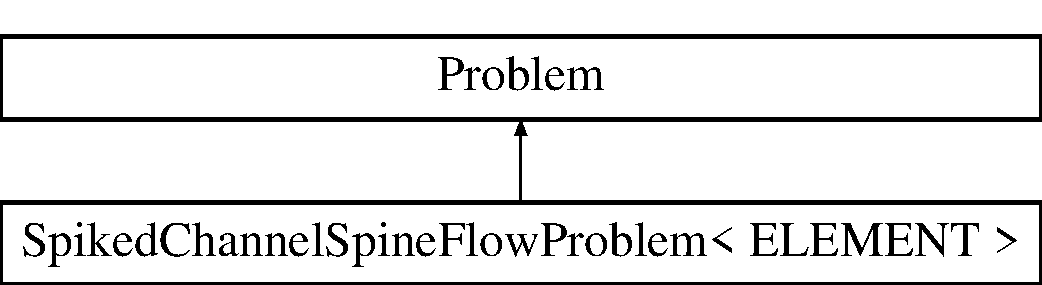
\includegraphics[height=2.000000cm]{classSpikedChannelSpineFlowProblem}
\end{center}
\end{figure}
\subsection*{Public Member Functions}
\begin{DoxyCompactItemize}
\item 
\hyperlink{classSpikedChannelSpineFlowProblem_a48ee634b61ca54658104d476c683264e}{$\sim$\+Spiked\+Channel\+Spine\+Flow\+Problem} ()
\begin{DoxyCompactList}\small\item\em Destructor\+: Empty. \end{DoxyCompactList}\item 
void \hyperlink{classSpikedChannelSpineFlowProblem_a4aca63a902ad477dbe1cb9d170aebbc2}{actions\+\_\+after\+\_\+newton\+\_\+solve} ()
\begin{DoxyCompactList}\small\item\em Update the after solve (empty) \end{DoxyCompactList}\item 
void \hyperlink{classSpikedChannelSpineFlowProblem_a98e464ea1ab1c14d703415d63e89115e}{actions\+\_\+before\+\_\+newton\+\_\+solve} ()
\begin{DoxyCompactList}\small\item\em Update the problem specs before solve. set velocity boundary conditions just to be on the safe side... \end{DoxyCompactList}\item 
Channel\+Spine\+Mesh$<$ E\+L\+E\+M\+E\+NT $>$ $\ast$ \hyperlink{classSpikedChannelSpineFlowProblem_a2125f8744b2e4a8f76a2bafee264db94}{mesh\+\_\+pt} ()
\begin{DoxyCompactList}\small\item\em Upcasted access function for the mesh. \end{DoxyCompactList}\item 
\hyperlink{classSpikedChannelSpineFlowProblem_a45f0bab84a0ecc00b7928d2e982af1bb}{Spiked\+Channel\+Spine\+Flow\+Problem} ()
\begin{DoxyCompactList}\small\item\em Constructor. \end{DoxyCompactList}\item 
void \hyperlink{classSpikedChannelSpineFlowProblem_ab9fc5d18831a928a3ad7e2e13efaa6c4}{doc\+\_\+solution} (Doc\+Info \&doc\+\_\+info)
\begin{DoxyCompactList}\small\item\em Doc the solution. \end{DoxyCompactList}\end{DoxyCompactItemize}
\subsection*{Private Attributes}
\begin{DoxyCompactItemize}
\item 
double \hyperlink{classSpikedChannelSpineFlowProblem_abb8d6a5648396f351835d646c2731b12}{Ly}
\begin{DoxyCompactList}\small\item\em Width of channel. \end{DoxyCompactList}\end{DoxyCompactItemize}


\subsection{Detailed Description}
\subsubsection*{template$<$class E\+L\+E\+M\+E\+NT$>$\newline
class Spiked\+Channel\+Spine\+Flow\+Problem$<$ E\+L\+E\+M\+E\+N\+T $>$}

Channel flow, through a non-\/uniform channel, using Spines. 

Definition at line 336 of file spine\+\_\+channel2.\+cc.



\subsection{Constructor \& Destructor Documentation}
\mbox{\Hypertarget{classSpikedChannelSpineFlowProblem_a48ee634b61ca54658104d476c683264e}\label{classSpikedChannelSpineFlowProblem_a48ee634b61ca54658104d476c683264e}} 
\index{Spiked\+Channel\+Spine\+Flow\+Problem@{Spiked\+Channel\+Spine\+Flow\+Problem}!````~Spiked\+Channel\+Spine\+Flow\+Problem@{$\sim$\+Spiked\+Channel\+Spine\+Flow\+Problem}}
\index{````~Spiked\+Channel\+Spine\+Flow\+Problem@{$\sim$\+Spiked\+Channel\+Spine\+Flow\+Problem}!Spiked\+Channel\+Spine\+Flow\+Problem@{Spiked\+Channel\+Spine\+Flow\+Problem}}
\subsubsection{\texorpdfstring{$\sim$\+Spiked\+Channel\+Spine\+Flow\+Problem()}{~SpikedChannelSpineFlowProblem()}}
{\footnotesize\ttfamily template$<$class E\+L\+E\+M\+E\+NT$>$ \\
\hyperlink{classSpikedChannelSpineFlowProblem}{Spiked\+Channel\+Spine\+Flow\+Problem}$<$ E\+L\+E\+M\+E\+NT $>$\+::$\sim$\hyperlink{classSpikedChannelSpineFlowProblem}{Spiked\+Channel\+Spine\+Flow\+Problem} (\begin{DoxyParamCaption}{ }\end{DoxyParamCaption})\hspace{0.3cm}{\ttfamily [inline]}}



Destructor\+: Empty. 



Definition at line 346 of file spine\+\_\+channel2.\+cc.

\mbox{\Hypertarget{classSpikedChannelSpineFlowProblem_a45f0bab84a0ecc00b7928d2e982af1bb}\label{classSpikedChannelSpineFlowProblem_a45f0bab84a0ecc00b7928d2e982af1bb}} 
\index{Spiked\+Channel\+Spine\+Flow\+Problem@{Spiked\+Channel\+Spine\+Flow\+Problem}!Spiked\+Channel\+Spine\+Flow\+Problem@{Spiked\+Channel\+Spine\+Flow\+Problem}}
\index{Spiked\+Channel\+Spine\+Flow\+Problem@{Spiked\+Channel\+Spine\+Flow\+Problem}!Spiked\+Channel\+Spine\+Flow\+Problem@{Spiked\+Channel\+Spine\+Flow\+Problem}}
\subsubsection{\texorpdfstring{Spiked\+Channel\+Spine\+Flow\+Problem()}{SpikedChannelSpineFlowProblem()}}
{\footnotesize\ttfamily template$<$class E\+L\+E\+M\+E\+NT $>$ \\
\hyperlink{classSpikedChannelSpineFlowProblem}{Spiked\+Channel\+Spine\+Flow\+Problem}$<$ E\+L\+E\+M\+E\+NT $>$\+::\hyperlink{classSpikedChannelSpineFlowProblem}{Spiked\+Channel\+Spine\+Flow\+Problem} (\begin{DoxyParamCaption}{ }\end{DoxyParamCaption})}



Constructor. 

Constructor for Spiked\+Channel\+Spine\+Flow problem 

Definition at line 417 of file spine\+\_\+channel2.\+cc.



References Global\+\_\+\+Physical\+\_\+\+Variables2\+::\+Re.



\subsection{Member Function Documentation}
\mbox{\Hypertarget{classSpikedChannelSpineFlowProblem_a4aca63a902ad477dbe1cb9d170aebbc2}\label{classSpikedChannelSpineFlowProblem_a4aca63a902ad477dbe1cb9d170aebbc2}} 
\index{Spiked\+Channel\+Spine\+Flow\+Problem@{Spiked\+Channel\+Spine\+Flow\+Problem}!actions\+\_\+after\+\_\+newton\+\_\+solve@{actions\+\_\+after\+\_\+newton\+\_\+solve}}
\index{actions\+\_\+after\+\_\+newton\+\_\+solve@{actions\+\_\+after\+\_\+newton\+\_\+solve}!Spiked\+Channel\+Spine\+Flow\+Problem@{Spiked\+Channel\+Spine\+Flow\+Problem}}
\subsubsection{\texorpdfstring{actions\+\_\+after\+\_\+newton\+\_\+solve()}{actions\_after\_newton\_solve()}}
{\footnotesize\ttfamily template$<$class E\+L\+E\+M\+E\+NT$>$ \\
void \hyperlink{classSpikedChannelSpineFlowProblem}{Spiked\+Channel\+Spine\+Flow\+Problem}$<$ E\+L\+E\+M\+E\+NT $>$\+::actions\+\_\+after\+\_\+newton\+\_\+solve (\begin{DoxyParamCaption}{ }\end{DoxyParamCaption})\hspace{0.3cm}{\ttfamily [inline]}}



Update the after solve (empty) 



Definition at line 349 of file spine\+\_\+channel2.\+cc.

\mbox{\Hypertarget{classSpikedChannelSpineFlowProblem_a98e464ea1ab1c14d703415d63e89115e}\label{classSpikedChannelSpineFlowProblem_a98e464ea1ab1c14d703415d63e89115e}} 
\index{Spiked\+Channel\+Spine\+Flow\+Problem@{Spiked\+Channel\+Spine\+Flow\+Problem}!actions\+\_\+before\+\_\+newton\+\_\+solve@{actions\+\_\+before\+\_\+newton\+\_\+solve}}
\index{actions\+\_\+before\+\_\+newton\+\_\+solve@{actions\+\_\+before\+\_\+newton\+\_\+solve}!Spiked\+Channel\+Spine\+Flow\+Problem@{Spiked\+Channel\+Spine\+Flow\+Problem}}
\subsubsection{\texorpdfstring{actions\+\_\+before\+\_\+newton\+\_\+solve()}{actions\_before\_newton\_solve()}}
{\footnotesize\ttfamily template$<$class E\+L\+E\+M\+E\+NT$>$ \\
void \hyperlink{classSpikedChannelSpineFlowProblem}{Spiked\+Channel\+Spine\+Flow\+Problem}$<$ E\+L\+E\+M\+E\+NT $>$\+::actions\+\_\+before\+\_\+newton\+\_\+solve (\begin{DoxyParamCaption}{ }\end{DoxyParamCaption})\hspace{0.3cm}{\ttfamily [inline]}}



Update the problem specs before solve. set velocity boundary conditions just to be on the safe side... 



Definition at line 353 of file spine\+\_\+channel2.\+cc.

\mbox{\Hypertarget{classSpikedChannelSpineFlowProblem_ab9fc5d18831a928a3ad7e2e13efaa6c4}\label{classSpikedChannelSpineFlowProblem_ab9fc5d18831a928a3ad7e2e13efaa6c4}} 
\index{Spiked\+Channel\+Spine\+Flow\+Problem@{Spiked\+Channel\+Spine\+Flow\+Problem}!doc\+\_\+solution@{doc\+\_\+solution}}
\index{doc\+\_\+solution@{doc\+\_\+solution}!Spiked\+Channel\+Spine\+Flow\+Problem@{Spiked\+Channel\+Spine\+Flow\+Problem}}
\subsubsection{\texorpdfstring{doc\+\_\+solution()}{doc\_solution()}}
{\footnotesize\ttfamily template$<$class E\+L\+E\+M\+E\+NT $>$ \\
void \hyperlink{classSpikedChannelSpineFlowProblem}{Spiked\+Channel\+Spine\+Flow\+Problem}$<$ E\+L\+E\+M\+E\+NT $>$\+::doc\+\_\+solution (\begin{DoxyParamCaption}\item[{Doc\+Info \&}]{doc\+\_\+info }\end{DoxyParamCaption})}



Doc the solution. 



Definition at line 503 of file spine\+\_\+channel2.\+cc.



Referenced by main().

\mbox{\Hypertarget{classSpikedChannelSpineFlowProblem_a2125f8744b2e4a8f76a2bafee264db94}\label{classSpikedChannelSpineFlowProblem_a2125f8744b2e4a8f76a2bafee264db94}} 
\index{Spiked\+Channel\+Spine\+Flow\+Problem@{Spiked\+Channel\+Spine\+Flow\+Problem}!mesh\+\_\+pt@{mesh\+\_\+pt}}
\index{mesh\+\_\+pt@{mesh\+\_\+pt}!Spiked\+Channel\+Spine\+Flow\+Problem@{Spiked\+Channel\+Spine\+Flow\+Problem}}
\subsubsection{\texorpdfstring{mesh\+\_\+pt()}{mesh\_pt()}}
{\footnotesize\ttfamily template$<$class E\+L\+E\+M\+E\+NT$>$ \\
Channel\+Spine\+Mesh$<$E\+L\+E\+M\+E\+NT$>$$\ast$ \hyperlink{classSpikedChannelSpineFlowProblem}{Spiked\+Channel\+Spine\+Flow\+Problem}$<$ E\+L\+E\+M\+E\+NT $>$\+::mesh\+\_\+pt (\begin{DoxyParamCaption}{ }\end{DoxyParamCaption})\hspace{0.3cm}{\ttfamily [inline]}}



Upcasted access function for the mesh. 



Definition at line 397 of file spine\+\_\+channel2.\+cc.



\subsection{Member Data Documentation}
\mbox{\Hypertarget{classSpikedChannelSpineFlowProblem_abb8d6a5648396f351835d646c2731b12}\label{classSpikedChannelSpineFlowProblem_abb8d6a5648396f351835d646c2731b12}} 
\index{Spiked\+Channel\+Spine\+Flow\+Problem@{Spiked\+Channel\+Spine\+Flow\+Problem}!Ly@{Ly}}
\index{Ly@{Ly}!Spiked\+Channel\+Spine\+Flow\+Problem@{Spiked\+Channel\+Spine\+Flow\+Problem}}
\subsubsection{\texorpdfstring{Ly}{Ly}}
{\footnotesize\ttfamily template$<$class E\+L\+E\+M\+E\+NT$>$ \\
double \hyperlink{classSpikedChannelSpineFlowProblem}{Spiked\+Channel\+Spine\+Flow\+Problem}$<$ E\+L\+E\+M\+E\+NT $>$\+::Ly\hspace{0.3cm}{\ttfamily [private]}}



Width of channel. 



Definition at line 341 of file spine\+\_\+channel2.\+cc.



The documentation for this class was generated from the following file\+:\begin{DoxyCompactItemize}
\item 
\hyperlink{spine__channel2_8cc}{spine\+\_\+channel2.\+cc}\end{DoxyCompactItemize}

\hypertarget{classSpikedLine}{}\section{Spiked\+Line Class Reference}
\label{classSpikedLine}\index{Spiked\+Line@{Spiked\+Line}}
Inheritance diagram for Spiked\+Line\+:\begin{figure}[H]
\begin{center}
\leavevmode
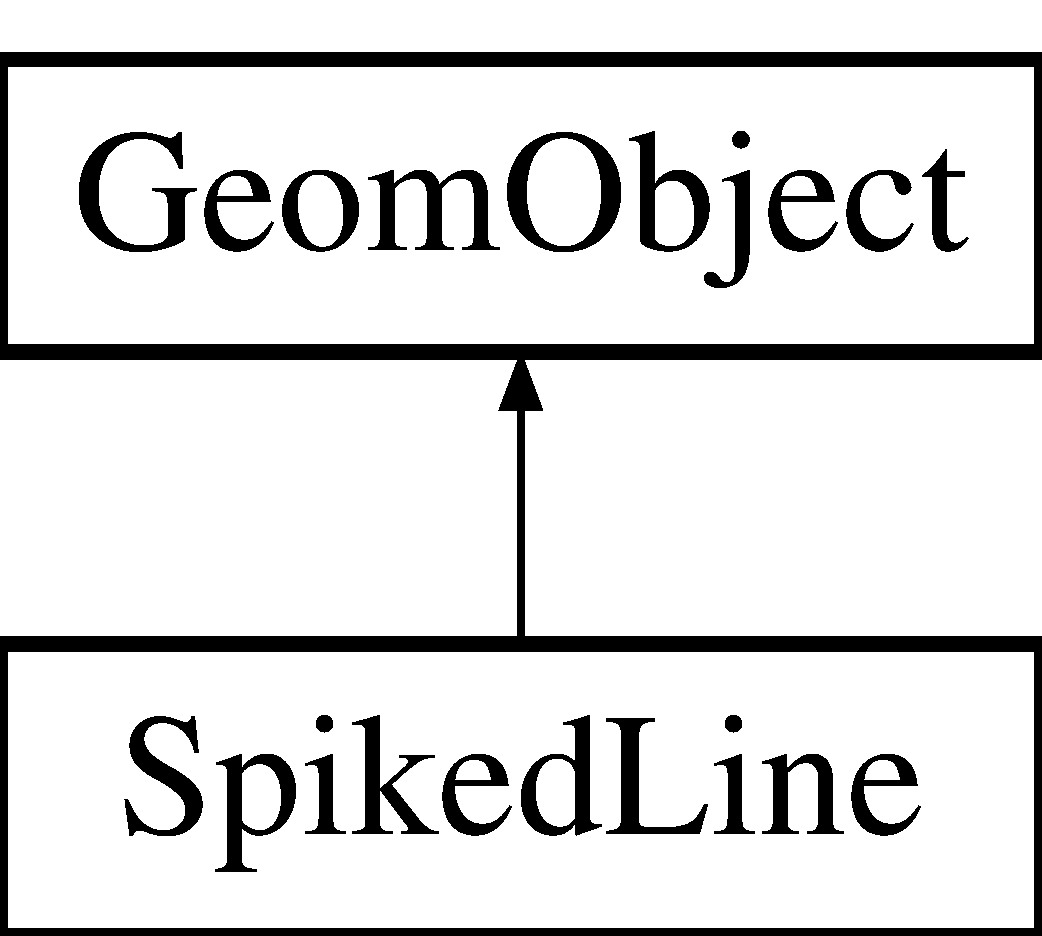
\includegraphics[height=2.000000cm]{classSpikedLine}
\end{center}
\end{figure}
\subsection*{Public Member Functions}
\begin{DoxyCompactItemize}
\item 
\hyperlink{classSpikedLine_a79ca76b80aebb0b32f63c125aee9d04d}{Spiked\+Line} (const Vector$<$ Data $\ast$$>$ \&\hyperlink{classSpikedLine_abf25117b43790ca3a9afb826188bc5fc}{geom\+\_\+data\+\_\+pt})
\begin{DoxyCompactList}\small\item\em Constructor\+: Four item of geometric data\+: \end{DoxyCompactList}\item 
\hyperlink{classSpikedLine_ad007f4c54d091b1c4ddb4b63cef0e7b6}{Spiked\+Line} (const double \&height, const double \&amplitude, const double \&zeta\+\_\+min, const double \&zeta\+\_\+max)
\begin{DoxyCompactList}\small\item\em Constructor\+: Pass height, amplitude, zeta min and zeta max (all are pinned by default) \end{DoxyCompactList}\item 
\hyperlink{classSpikedLine_a54f1b8a7951ad8205741e78fc75afaa3}{$\sim$\+Spiked\+Line} ()
\begin{DoxyCompactList}\small\item\em Destructor\+: Clean up if necessary. \end{DoxyCompactList}\item 
void \hyperlink{classSpikedLine_a11a6078a409096caaf21dd56b97e1528}{position} (const Vector$<$ double $>$ \&zeta, Vector$<$ double $>$ \&r) const
\begin{DoxyCompactList}\small\item\em Position Vector at Lagrangian coordinate zeta. \end{DoxyCompactList}\item 
void \hyperlink{classSpikedLine_ac6356a30cad06346e46a494e226d5219}{position} (const unsigned \&t, const Vector$<$ double $>$ \&zeta, Vector$<$ double $>$ \&r) const
\begin{DoxyCompactList}\small\item\em Parametrised position on object\+: r(zeta). Evaluated at previous timestep. t=0\+: current time; t$>$0\+: previous timestep. \end{DoxyCompactList}\item 
virtual void \hyperlink{classSpikedLine_a8c7c95b0c572a33ca9206b01d10c99c5}{dposition} (const Vector$<$ double $>$ \&zeta, Dense\+Matrix$<$ double $>$ \&drdzeta) const
\begin{DoxyCompactList}\small\item\em Derivative of position Vector w.\+r.\+t. to coordinates\+: $ \frac{dR_i}{d \zeta_\alpha}$ = drdzeta(alpha,i). Evaluated at current time. \end{DoxyCompactList}\item 
virtual void \hyperlink{classSpikedLine_a5feeb76bcde12139b4fc5b8797ae033b}{d2position} (const Vector$<$ double $>$ \&zeta, Rank\+Three\+Tensor$<$ double $>$ \&ddrdzeta) const
\begin{DoxyCompactList}\small\item\em 2nd derivative of position Vector w.\+r.\+t. to coordinates\+: $ \frac{d^2R_i}{d \zeta_\alpha d \zeta_\beta}$ = ddrdzeta(alpha,beta,i). Evaluated at current time. \end{DoxyCompactList}\item 
virtual void \hyperlink{classSpikedLine_a1f670bc6cc3aae65d209ecffb7a63ec2}{d2position} (const Vector$<$ double $>$ \&zeta, Vector$<$ double $>$ \&r, Dense\+Matrix$<$ double $>$ \&drdzeta, Rank\+Three\+Tensor$<$ double $>$ \&ddrdzeta) const
\begin{DoxyCompactList}\small\item\em Posn Vector and its 1st \& 2nd derivatives w.\+r.\+t. to coordinates\+: $ \frac{dR_i}{d \zeta_\alpha}$ = drdzeta(alpha,i). $ \frac{d^2R_i}{d \zeta_\alpha d \zeta_\beta}$ = ddrdzeta(alpha,beta,i). Evaluated at current time. \end{DoxyCompactList}\item 
unsigned \hyperlink{classSpikedLine_a13ef991b5c044d5f6ce154122c10aeca}{ngeom\+\_\+data} () const
\begin{DoxyCompactList}\small\item\em How many items of Data does the shape of the object depend on? \end{DoxyCompactList}\item 
Data $\ast$ \hyperlink{classSpikedLine_abf25117b43790ca3a9afb826188bc5fc}{geom\+\_\+data\+\_\+pt} (const unsigned \&j)
\begin{DoxyCompactList}\small\item\em Return pointer to the j-\/th Data item that the object\textquotesingle{}s shape depends on. \end{DoxyCompactList}\end{DoxyCompactItemize}
\subsection*{Private Attributes}
\begin{DoxyCompactItemize}
\item 
Vector$<$ Data $\ast$ $>$ \hyperlink{classSpikedLine_a62f6dbf18fd631df474089e41ae7afeb}{Geom\+\_\+data\+\_\+pt}
\begin{DoxyCompactList}\small\item\em Vector of pointers to Data items that affects the object\textquotesingle{}s shape. \end{DoxyCompactList}\item 
bool \hyperlink{classSpikedLine_a4ac7004ff4f8417640ad07ad32b9c9e0}{Must\+\_\+clean\+\_\+up}
\begin{DoxyCompactList}\small\item\em Do I need to clean up? \end{DoxyCompactList}\end{DoxyCompactItemize}


\subsection{Detailed Description}
Steady, spiked 1D line in 2D space \[ x = \zeta \] \[ y = \left\{ \begin{array}{cl} H + 2A\left(\frac{\zeta - \zeta_{\mbox{min}}} {\zeta_{\mbox{max}} - \zeta_{\mbox{min}}}\right) & \mbox{for } \zeta \leq \frac{1}{2} \left(\zeta_{\mbox{max}} + \zeta_{\mbox{min}}\right)\\H + 2A\left(\frac{\zeta - \zeta_{\mbox{max}}} {\zeta_{\mbox{min}} - \zeta_{\mbox{max}}}\right) & \mbox{for } \zeta > \frac{1}{2} \left(\zeta_{\mbox{max}} + \zeta_{\mbox{min}}\right)\\ \end{array} \right.\] 

Definition at line 80 of file spine\+\_\+channel2.\+cc.



\subsection{Constructor \& Destructor Documentation}
\mbox{\Hypertarget{classSpikedLine_a79ca76b80aebb0b32f63c125aee9d04d}\label{classSpikedLine_a79ca76b80aebb0b32f63c125aee9d04d}} 
\index{Spiked\+Line@{Spiked\+Line}!Spiked\+Line@{Spiked\+Line}}
\index{Spiked\+Line@{Spiked\+Line}!Spiked\+Line@{Spiked\+Line}}
\subsubsection{\texorpdfstring{Spiked\+Line()}{SpikedLine()}\hspace{0.1cm}{\footnotesize\ttfamily [1/2]}}
{\footnotesize\ttfamily Spiked\+Line\+::\+Spiked\+Line (\begin{DoxyParamCaption}\item[{const Vector$<$ Data $\ast$$>$ \&}]{geom\+\_\+data\+\_\+pt }\end{DoxyParamCaption})\hspace{0.3cm}{\ttfamily [inline]}}



Constructor\+: Four item of geometric data\+: 


\begin{DoxyCode}
\hyperlink{classSpikedLine_a62f6dbf18fd631df474089e41ae7afeb}{Geom\_data\_pt}[0]->value(0) = \hyperlink{namespaceGlobal__Physical__Variables_aad3f0468efff43e7f235a64c27d3acf2}{height}
\hyperlink{classSpikedLine_a62f6dbf18fd631df474089e41ae7afeb}{Geom\_data\_pt}[0]->value(1) = amplitude
\hyperlink{classSpikedLine_a62f6dbf18fd631df474089e41ae7afeb}{Geom\_data\_pt}[0]->value(2) = zeta\_min
\hyperlink{classSpikedLine_a62f6dbf18fd631df474089e41ae7afeb}{Geom\_data\_pt}[0]->value(3) = zeta\_max
\end{DoxyCode}
 

Definition at line 92 of file spine\+\_\+channel2.\+cc.

\mbox{\Hypertarget{classSpikedLine_ad007f4c54d091b1c4ddb4b63cef0e7b6}\label{classSpikedLine_ad007f4c54d091b1c4ddb4b63cef0e7b6}} 
\index{Spiked\+Line@{Spiked\+Line}!Spiked\+Line@{Spiked\+Line}}
\index{Spiked\+Line@{Spiked\+Line}!Spiked\+Line@{Spiked\+Line}}
\subsubsection{\texorpdfstring{Spiked\+Line()}{SpikedLine()}\hspace{0.1cm}{\footnotesize\ttfamily [2/2]}}
{\footnotesize\ttfamily Spiked\+Line\+::\+Spiked\+Line (\begin{DoxyParamCaption}\item[{const double \&}]{height,  }\item[{const double \&}]{amplitude,  }\item[{const double \&}]{zeta\+\_\+min,  }\item[{const double \&}]{zeta\+\_\+max }\end{DoxyParamCaption})\hspace{0.3cm}{\ttfamily [inline]}}



Constructor\+: Pass height, amplitude, zeta min and zeta max (all are pinned by default) 



Definition at line 121 of file spine\+\_\+channel2.\+cc.

\mbox{\Hypertarget{classSpikedLine_a54f1b8a7951ad8205741e78fc75afaa3}\label{classSpikedLine_a54f1b8a7951ad8205741e78fc75afaa3}} 
\index{Spiked\+Line@{Spiked\+Line}!````~Spiked\+Line@{$\sim$\+Spiked\+Line}}
\index{````~Spiked\+Line@{$\sim$\+Spiked\+Line}!Spiked\+Line@{Spiked\+Line}}
\subsubsection{\texorpdfstring{$\sim$\+Spiked\+Line()}{~SpikedLine()}}
{\footnotesize\ttfamily Spiked\+Line\+::$\sim$\+Spiked\+Line (\begin{DoxyParamCaption}{ }\end{DoxyParamCaption})\hspace{0.3cm}{\ttfamily [inline]}}



Destructor\+: Clean up if necessary. 



Definition at line 146 of file spine\+\_\+channel2.\+cc.



\subsection{Member Function Documentation}
\mbox{\Hypertarget{classSpikedLine_a5feeb76bcde12139b4fc5b8797ae033b}\label{classSpikedLine_a5feeb76bcde12139b4fc5b8797ae033b}} 
\index{Spiked\+Line@{Spiked\+Line}!d2position@{d2position}}
\index{d2position@{d2position}!Spiked\+Line@{Spiked\+Line}}
\subsubsection{\texorpdfstring{d2position()}{d2position()}\hspace{0.1cm}{\footnotesize\ttfamily [1/2]}}
{\footnotesize\ttfamily virtual void Spiked\+Line\+::d2position (\begin{DoxyParamCaption}\item[{const Vector$<$ double $>$ \&}]{zeta,  }\item[{Rank\+Three\+Tensor$<$ double $>$ \&}]{ddrdzeta }\end{DoxyParamCaption}) const\hspace{0.3cm}{\ttfamily [inline]}, {\ttfamily [virtual]}}



2nd derivative of position Vector w.\+r.\+t. to coordinates\+: $ \frac{d^2R_i}{d \zeta_\alpha d \zeta_\beta}$ = ddrdzeta(alpha,beta,i). Evaluated at current time. 



Definition at line 256 of file spine\+\_\+channel2.\+cc.

\mbox{\Hypertarget{classSpikedLine_a1f670bc6cc3aae65d209ecffb7a63ec2}\label{classSpikedLine_a1f670bc6cc3aae65d209ecffb7a63ec2}} 
\index{Spiked\+Line@{Spiked\+Line}!d2position@{d2position}}
\index{d2position@{d2position}!Spiked\+Line@{Spiked\+Line}}
\subsubsection{\texorpdfstring{d2position()}{d2position()}\hspace{0.1cm}{\footnotesize\ttfamily [2/2]}}
{\footnotesize\ttfamily virtual void Spiked\+Line\+::d2position (\begin{DoxyParamCaption}\item[{const Vector$<$ double $>$ \&}]{zeta,  }\item[{Vector$<$ double $>$ \&}]{r,  }\item[{Dense\+Matrix$<$ double $>$ \&}]{drdzeta,  }\item[{Rank\+Three\+Tensor$<$ double $>$ \&}]{ddrdzeta }\end{DoxyParamCaption}) const\hspace{0.3cm}{\ttfamily [inline]}, {\ttfamily [virtual]}}



Posn Vector and its 1st \& 2nd derivatives w.\+r.\+t. to coordinates\+: $ \frac{dR_i}{d \zeta_\alpha}$ = drdzeta(alpha,i). $ \frac{d^2R_i}{d \zeta_\alpha d \zeta_\beta}$ = ddrdzeta(alpha,beta,i). Evaluated at current time. 



Definition at line 270 of file spine\+\_\+channel2.\+cc.



References Global\+\_\+\+Physical\+\_\+\+Variables\+::A, and Global\+\_\+\+Physical\+\_\+\+Variables\+::H.

\mbox{\Hypertarget{classSpikedLine_a8c7c95b0c572a33ca9206b01d10c99c5}\label{classSpikedLine_a8c7c95b0c572a33ca9206b01d10c99c5}} 
\index{Spiked\+Line@{Spiked\+Line}!dposition@{dposition}}
\index{dposition@{dposition}!Spiked\+Line@{Spiked\+Line}}
\subsubsection{\texorpdfstring{dposition()}{dposition()}}
{\footnotesize\ttfamily virtual void Spiked\+Line\+::dposition (\begin{DoxyParamCaption}\item[{const Vector$<$ double $>$ \&}]{zeta,  }\item[{Dense\+Matrix$<$ double $>$ \&}]{drdzeta }\end{DoxyParamCaption}) const\hspace{0.3cm}{\ttfamily [inline]}, {\ttfamily [virtual]}}



Derivative of position Vector w.\+r.\+t. to coordinates\+: $ \frac{dR_i}{d \zeta_\alpha}$ = drdzeta(alpha,i). Evaluated at current time. 



Definition at line 231 of file spine\+\_\+channel2.\+cc.



References Global\+\_\+\+Physical\+\_\+\+Variables\+::A.

\mbox{\Hypertarget{classSpikedLine_abf25117b43790ca3a9afb826188bc5fc}\label{classSpikedLine_abf25117b43790ca3a9afb826188bc5fc}} 
\index{Spiked\+Line@{Spiked\+Line}!geom\+\_\+data\+\_\+pt@{geom\+\_\+data\+\_\+pt}}
\index{geom\+\_\+data\+\_\+pt@{geom\+\_\+data\+\_\+pt}!Spiked\+Line@{Spiked\+Line}}
\subsubsection{\texorpdfstring{geom\+\_\+data\+\_\+pt()}{geom\_data\_pt()}}
{\footnotesize\ttfamily Data$\ast$ Spiked\+Line\+::geom\+\_\+data\+\_\+pt (\begin{DoxyParamCaption}\item[{const unsigned \&}]{j }\end{DoxyParamCaption})\hspace{0.3cm}{\ttfamily [inline]}}



Return pointer to the j-\/th Data item that the object\textquotesingle{}s shape depends on. 



Definition at line 313 of file spine\+\_\+channel2.\+cc.

\mbox{\Hypertarget{classSpikedLine_a13ef991b5c044d5f6ce154122c10aeca}\label{classSpikedLine_a13ef991b5c044d5f6ce154122c10aeca}} 
\index{Spiked\+Line@{Spiked\+Line}!ngeom\+\_\+data@{ngeom\+\_\+data}}
\index{ngeom\+\_\+data@{ngeom\+\_\+data}!Spiked\+Line@{Spiked\+Line}}
\subsubsection{\texorpdfstring{ngeom\+\_\+data()}{ngeom\_data()}}
{\footnotesize\ttfamily unsigned Spiked\+Line\+::ngeom\+\_\+data (\begin{DoxyParamCaption}{ }\end{DoxyParamCaption}) const\hspace{0.3cm}{\ttfamily [inline]}}



How many items of Data does the shape of the object depend on? 



Definition at line 309 of file spine\+\_\+channel2.\+cc.

\mbox{\Hypertarget{classSpikedLine_a11a6078a409096caaf21dd56b97e1528}\label{classSpikedLine_a11a6078a409096caaf21dd56b97e1528}} 
\index{Spiked\+Line@{Spiked\+Line}!position@{position}}
\index{position@{position}!Spiked\+Line@{Spiked\+Line}}
\subsubsection{\texorpdfstring{position()}{position()}\hspace{0.1cm}{\footnotesize\ttfamily [1/2]}}
{\footnotesize\ttfamily void Spiked\+Line\+::position (\begin{DoxyParamCaption}\item[{const Vector$<$ double $>$ \&}]{zeta,  }\item[{Vector$<$ double $>$ \&}]{r }\end{DoxyParamCaption}) const\hspace{0.3cm}{\ttfamily [inline]}}



Position Vector at Lagrangian coordinate zeta. 



Definition at line 158 of file spine\+\_\+channel2.\+cc.



References Global\+\_\+\+Physical\+\_\+\+Variables\+::A, and Global\+\_\+\+Physical\+\_\+\+Variables\+::H.

\mbox{\Hypertarget{classSpikedLine_ac6356a30cad06346e46a494e226d5219}\label{classSpikedLine_ac6356a30cad06346e46a494e226d5219}} 
\index{Spiked\+Line@{Spiked\+Line}!position@{position}}
\index{position@{position}!Spiked\+Line@{Spiked\+Line}}
\subsubsection{\texorpdfstring{position()}{position()}\hspace{0.1cm}{\footnotesize\ttfamily [2/2]}}
{\footnotesize\ttfamily void Spiked\+Line\+::position (\begin{DoxyParamCaption}\item[{const unsigned \&}]{t,  }\item[{const Vector$<$ double $>$ \&}]{zeta,  }\item[{Vector$<$ double $>$ \&}]{r }\end{DoxyParamCaption}) const\hspace{0.3cm}{\ttfamily [inline]}}



Parametrised position on object\+: r(zeta). Evaluated at previous timestep. t=0\+: current time; t$>$0\+: previous timestep. 



Definition at line 191 of file spine\+\_\+channel2.\+cc.



References Global\+\_\+\+Physical\+\_\+\+Variables\+::A, and Global\+\_\+\+Physical\+\_\+\+Variables\+::H.



\subsection{Member Data Documentation}
\mbox{\Hypertarget{classSpikedLine_a62f6dbf18fd631df474089e41ae7afeb}\label{classSpikedLine_a62f6dbf18fd631df474089e41ae7afeb}} 
\index{Spiked\+Line@{Spiked\+Line}!Geom\+\_\+data\+\_\+pt@{Geom\+\_\+data\+\_\+pt}}
\index{Geom\+\_\+data\+\_\+pt@{Geom\+\_\+data\+\_\+pt}!Spiked\+Line@{Spiked\+Line}}
\subsubsection{\texorpdfstring{Geom\+\_\+data\+\_\+pt}{Geom\_data\_pt}}
{\footnotesize\ttfamily Vector$<$Data$\ast$$>$ Spiked\+Line\+::\+Geom\+\_\+data\+\_\+pt\hspace{0.3cm}{\ttfamily [private]}}



Vector of pointers to Data items that affects the object\textquotesingle{}s shape. 



Definition at line 319 of file spine\+\_\+channel2.\+cc.

\mbox{\Hypertarget{classSpikedLine_a4ac7004ff4f8417640ad07ad32b9c9e0}\label{classSpikedLine_a4ac7004ff4f8417640ad07ad32b9c9e0}} 
\index{Spiked\+Line@{Spiked\+Line}!Must\+\_\+clean\+\_\+up@{Must\+\_\+clean\+\_\+up}}
\index{Must\+\_\+clean\+\_\+up@{Must\+\_\+clean\+\_\+up}!Spiked\+Line@{Spiked\+Line}}
\subsubsection{\texorpdfstring{Must\+\_\+clean\+\_\+up}{Must\_clean\_up}}
{\footnotesize\ttfamily bool Spiked\+Line\+::\+Must\+\_\+clean\+\_\+up\hspace{0.3cm}{\ttfamily [private]}}



Do I need to clean up? 



Definition at line 322 of file spine\+\_\+channel2.\+cc.



The documentation for this class was generated from the following file\+:\begin{DoxyCompactItemize}
\item 
\hyperlink{spine__channel2_8cc}{spine\+\_\+channel2.\+cc}\end{DoxyCompactItemize}

\hypertarget{classWavyWall}{}\section{Wavy\+Wall Class Reference}
\label{classWavyWall}\index{Wavy\+Wall@{Wavy\+Wall}}
Inheritance diagram for Wavy\+Wall\+:\begin{figure}[H]
\begin{center}
\leavevmode
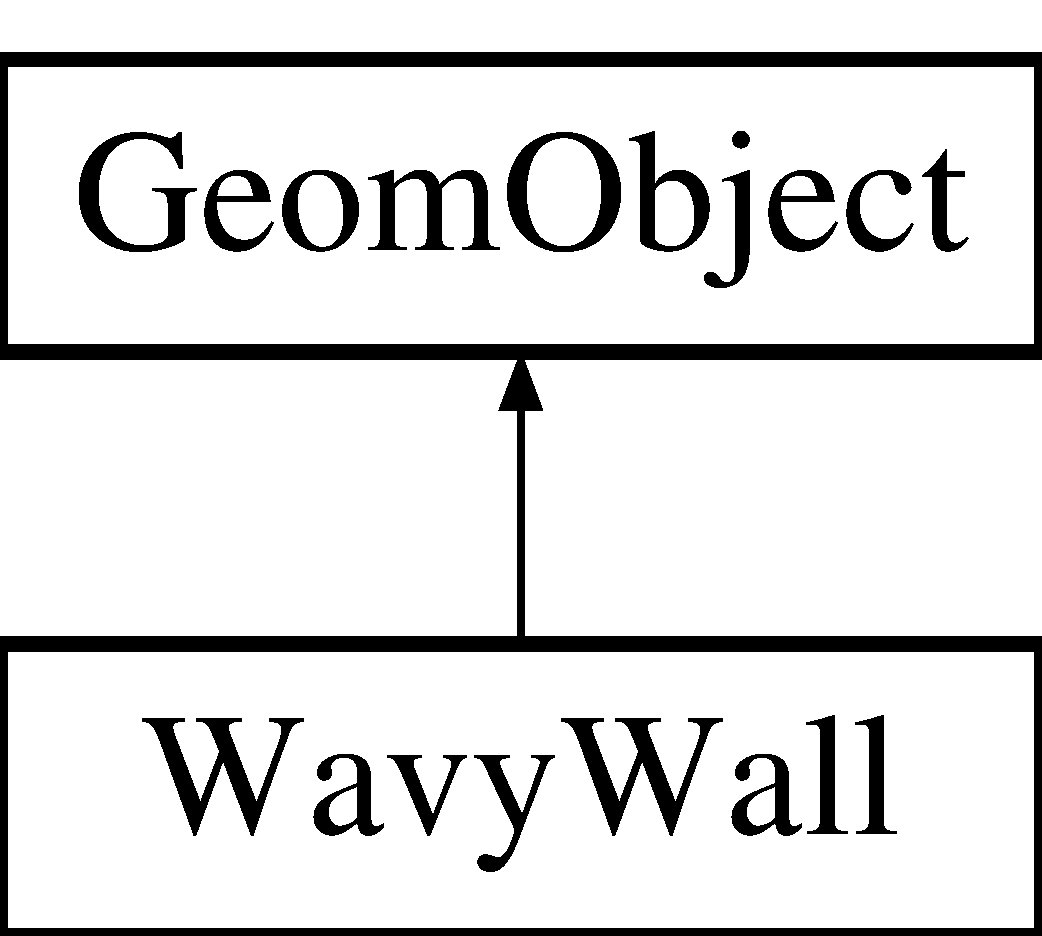
\includegraphics[height=2.000000cm]{classWavyWall}
\end{center}
\end{figure}
\subsection*{Public Member Functions}
\begin{DoxyCompactItemize}
\item 
\hyperlink{classWavyWall_a7ef7a36cbce8798c1e4a99165dee8cc0}{Wavy\+Wall} (const double \&l, const double \&amplitude)
\begin{DoxyCompactList}\small\item\em Constructor\+: Pass wavelength and amplitude. \end{DoxyCompactList}\item 
void \hyperlink{classWavyWall_a9a9f5a98cb0d15ee801b52495be5e5bf}{position} (const Vector$<$ double $>$ \&zeta, Vector$<$ double $>$ \&r) const
\begin{DoxyCompactList}\small\item\em Position vector to wavy wall. \end{DoxyCompactList}\end{DoxyCompactItemize}
\subsection*{Protected Attributes}
\begin{DoxyCompactItemize}
\item 
double \hyperlink{classWavyWall_a598b42ece2600db9eb8c4d1dfeca9ad1}{L}
\begin{DoxyCompactList}\small\item\em Wavelength. \end{DoxyCompactList}\item 
double \hyperlink{classWavyWall_a435f0fb4db45b51eb371b66b244c7630}{A}
\begin{DoxyCompactList}\small\item\em Amplitude. \end{DoxyCompactList}\end{DoxyCompactItemize}


\subsection{Detailed Description}
Geometric object representing a wavy wall, parametrised by \[ x = \zeta \] \[ y = A (1 - \cos(2\pi\zeta/L) )\] 

Definition at line 56 of file simple\+\_\+spine\+\_\+channel.\+cc.



\subsection{Constructor \& Destructor Documentation}
\mbox{\Hypertarget{classWavyWall_a7ef7a36cbce8798c1e4a99165dee8cc0}\label{classWavyWall_a7ef7a36cbce8798c1e4a99165dee8cc0}} 
\index{Wavy\+Wall@{Wavy\+Wall}!Wavy\+Wall@{Wavy\+Wall}}
\index{Wavy\+Wall@{Wavy\+Wall}!Wavy\+Wall@{Wavy\+Wall}}
\subsubsection{\texorpdfstring{Wavy\+Wall()}{WavyWall()}}
{\footnotesize\ttfamily Wavy\+Wall\+::\+Wavy\+Wall (\begin{DoxyParamCaption}\item[{const double \&}]{l,  }\item[{const double \&}]{amplitude }\end{DoxyParamCaption})\hspace{0.3cm}{\ttfamily [inline]}}



Constructor\+: Pass wavelength and amplitude. 



Definition at line 62 of file simple\+\_\+spine\+\_\+channel.\+cc.



\subsection{Member Function Documentation}
\mbox{\Hypertarget{classWavyWall_a9a9f5a98cb0d15ee801b52495be5e5bf}\label{classWavyWall_a9a9f5a98cb0d15ee801b52495be5e5bf}} 
\index{Wavy\+Wall@{Wavy\+Wall}!position@{position}}
\index{position@{position}!Wavy\+Wall@{Wavy\+Wall}}
\subsubsection{\texorpdfstring{position()}{position()}}
{\footnotesize\ttfamily void Wavy\+Wall\+::position (\begin{DoxyParamCaption}\item[{const Vector$<$ double $>$ \&}]{zeta,  }\item[{Vector$<$ double $>$ \&}]{r }\end{DoxyParamCaption}) const\hspace{0.3cm}{\ttfamily [inline]}}



Position vector to wavy wall. 



Definition at line 66 of file simple\+\_\+spine\+\_\+channel.\+cc.



References Global\+\_\+\+Physical\+\_\+\+Variables\+::A, and Global\+\_\+\+Physical\+\_\+\+Variables\+::L.



\subsection{Member Data Documentation}
\mbox{\Hypertarget{classWavyWall_a435f0fb4db45b51eb371b66b244c7630}\label{classWavyWall_a435f0fb4db45b51eb371b66b244c7630}} 
\index{Wavy\+Wall@{Wavy\+Wall}!A@{A}}
\index{A@{A}!Wavy\+Wall@{Wavy\+Wall}}
\subsubsection{\texorpdfstring{A}{A}}
{\footnotesize\ttfamily double Wavy\+Wall\+::A\hspace{0.3cm}{\ttfamily [protected]}}



Amplitude. 



Definition at line 78 of file simple\+\_\+spine\+\_\+channel.\+cc.

\mbox{\Hypertarget{classWavyWall_a598b42ece2600db9eb8c4d1dfeca9ad1}\label{classWavyWall_a598b42ece2600db9eb8c4d1dfeca9ad1}} 
\index{Wavy\+Wall@{Wavy\+Wall}!L@{L}}
\index{L@{L}!Wavy\+Wall@{Wavy\+Wall}}
\subsubsection{\texorpdfstring{L}{L}}
{\footnotesize\ttfamily double Wavy\+Wall\+::L\hspace{0.3cm}{\ttfamily [protected]}}



Wavelength. 



Definition at line 75 of file simple\+\_\+spine\+\_\+channel.\+cc.



The documentation for this class was generated from the following file\+:\begin{DoxyCompactItemize}
\item 
\hyperlink{simple__spine__channel_8cc}{simple\+\_\+spine\+\_\+channel.\+cc}\end{DoxyCompactItemize}

\chapter{File Documentation}
\hypertarget{simple__spine__channel_8cc}{}\section{simple\+\_\+spine\+\_\+channel.\+cc File Reference}
\label{simple__spine__channel_8cc}\index{simple\+\_\+spine\+\_\+channel.\+cc@{simple\+\_\+spine\+\_\+channel.\+cc}}
\subsection*{Classes}
\begin{DoxyCompactItemize}
\item 
class \hyperlink{classWavyWall}{Wavy\+Wall}
\item 
class \hyperlink{classSimpleSpineMesh}{Simple\+Spine\+Mesh$<$ E\+L\+E\+M\+E\+N\+T $>$}
\item 
class \hyperlink{classChannelSpineFlowProblem}{Channel\+Spine\+Flow\+Problem$<$ E\+L\+E\+M\+E\+N\+T $>$}
\end{DoxyCompactItemize}
\subsection*{Namespaces}
\begin{DoxyCompactItemize}
\item 
 \hyperlink{namespaceGlobal__Physical__Variables}{Global\+\_\+\+Physical\+\_\+\+Variables}
\begin{DoxyCompactList}\small\item\em Namespace for physical parameters. \end{DoxyCompactList}\end{DoxyCompactItemize}
\subsection*{Functions}
\begin{DoxyCompactItemize}
\item 
double \hyperlink{namespaceGlobal__Physical__Variables_aad3f0468efff43e7f235a64c27d3acf2}{Global\+\_\+\+Physical\+\_\+\+Variables\+::height} (const double \&x)
\begin{DoxyCompactList}\small\item\em Height of domain. \end{DoxyCompactList}\item 
int \hyperlink{simple__spine__channel_8cc_ae66f6b31b5ad750f1fe042a706a4e3d4}{main} ()
\begin{DoxyCompactList}\small\item\em Driver for channel flow problem with spine mesh. \end{DoxyCompactList}\end{DoxyCompactItemize}
\subsection*{Variables}
\begin{DoxyCompactItemize}
\item 
double \hyperlink{namespaceGlobal__Physical__Variables_ab814e627d2eb5bc50318879d19ab16b9}{Global\+\_\+\+Physical\+\_\+\+Variables\+::\+Re} =100
\begin{DoxyCompactList}\small\item\em Reynolds number. \end{DoxyCompactList}\item 
double \hyperlink{namespaceGlobal__Physical__Variables_a84cf50616e15acc4db0d9d8765302128}{Global\+\_\+\+Physical\+\_\+\+Variables\+::\+X\+\_\+indent\+\_\+start} =0.\+5
\begin{DoxyCompactList}\small\item\em Start of indented region. \end{DoxyCompactList}\item 
double \hyperlink{namespaceGlobal__Physical__Variables_a1b8bfc451f6b7ac89eca18f04338f47f}{Global\+\_\+\+Physical\+\_\+\+Variables\+::L} =1.\+0
\begin{DoxyCompactList}\small\item\em Length of indented region. \end{DoxyCompactList}\item 
double \hyperlink{namespaceGlobal__Physical__Variables_a9ec945e33c27b1cfe2e4da7cf3a89f72}{Global\+\_\+\+Physical\+\_\+\+Variables\+::\+L\+\_\+total} =4.\+0
\begin{DoxyCompactList}\small\item\em Total length of domain. \end{DoxyCompactList}\item 
double \hyperlink{namespaceGlobal__Physical__Variables_af6e07423e22c0991084d9a2f43727805}{Global\+\_\+\+Physical\+\_\+\+Variables\+::H} =1.\+0
\begin{DoxyCompactList}\small\item\em Undeformed height of domain. \end{DoxyCompactList}\item 
double \hyperlink{namespaceGlobal__Physical__Variables_a4894f9a3a9cbf84f00d0719f2841e624}{Global\+\_\+\+Physical\+\_\+\+Variables\+::A} =-\/0.\+6
\begin{DoxyCompactList}\small\item\em Amplitude of indentation. \end{DoxyCompactList}\end{DoxyCompactItemize}


\subsection{Function Documentation}
\mbox{\Hypertarget{simple__spine__channel_8cc_ae66f6b31b5ad750f1fe042a706a4e3d4}\label{simple__spine__channel_8cc_ae66f6b31b5ad750f1fe042a706a4e3d4}} 
\index{simple\+\_\+spine\+\_\+channel.\+cc@{simple\+\_\+spine\+\_\+channel.\+cc}!main@{main}}
\index{main@{main}!simple\+\_\+spine\+\_\+channel.\+cc@{simple\+\_\+spine\+\_\+channel.\+cc}}
\subsubsection{\texorpdfstring{main()}{main()}}
{\footnotesize\ttfamily int main (\begin{DoxyParamCaption}{ }\end{DoxyParamCaption})}



Driver for channel flow problem with spine mesh. 



Definition at line 658 of file simple\+\_\+spine\+\_\+channel.\+cc.



References Channel\+Spine\+Flow\+Problem$<$ E\+L\+E\+M\+E\+N\+T $>$\+::doc\+\_\+solution().


\hypertarget{spine__channel_8cc}{}\section{spine\+\_\+channel.\+cc File Reference}
\label{spine__channel_8cc}\index{spine\+\_\+channel.\+cc@{spine\+\_\+channel.\+cc}}
\subsection*{Classes}
\begin{DoxyCompactItemize}
\item 
class \hyperlink{classSinusoidalWall}{Sinusoidal\+Wall}
\item 
class \hyperlink{classChannelSpineFlowProblem}{Channel\+Spine\+Flow\+Problem$<$ E\+L\+E\+M\+E\+N\+T $>$}
\end{DoxyCompactItemize}
\subsection*{Namespaces}
\begin{DoxyCompactItemize}
\item 
 \hyperlink{namespaceGlobal__Physical__Variables}{Global\+\_\+\+Physical\+\_\+\+Variables}
\begin{DoxyCompactList}\small\item\em Namespace for physical parameters. \end{DoxyCompactList}\end{DoxyCompactItemize}
\subsection*{Functions}
\begin{DoxyCompactItemize}
\item 
int \hyperlink{spine__channel_8cc_ae66f6b31b5ad750f1fe042a706a4e3d4}{main} ()
\begin{DoxyCompactList}\small\item\em Driver for channel flow problem with spine mesh. \end{DoxyCompactList}\item 
void \hyperlink{spine__channel_8cc_aafbeb01abdfa5fac0d1ec9211bc67010}{doc\+\_\+sparse\+\_\+node\+\_\+update} ()
\begin{DoxyCompactList}\small\item\em Create the files to illustrate the sparse node update operation. \end{DoxyCompactList}\end{DoxyCompactItemize}


\subsection{Function Documentation}
\mbox{\Hypertarget{spine__channel_8cc_aafbeb01abdfa5fac0d1ec9211bc67010}\label{spine__channel_8cc_aafbeb01abdfa5fac0d1ec9211bc67010}} 
\index{spine\+\_\+channel.\+cc@{spine\+\_\+channel.\+cc}!doc\+\_\+sparse\+\_\+node\+\_\+update@{doc\+\_\+sparse\+\_\+node\+\_\+update}}
\index{doc\+\_\+sparse\+\_\+node\+\_\+update@{doc\+\_\+sparse\+\_\+node\+\_\+update}!spine\+\_\+channel.\+cc@{spine\+\_\+channel.\+cc}}
\subsubsection{\texorpdfstring{doc\+\_\+sparse\+\_\+node\+\_\+update()}{doc\_sparse\_node\_update()}}
{\footnotesize\ttfamily void doc\+\_\+sparse\+\_\+node\+\_\+update (\begin{DoxyParamCaption}{ }\end{DoxyParamCaption})}



Create the files to illustrate the sparse node update operation. 



Definition at line 562 of file spine\+\_\+channel.\+cc.

\mbox{\Hypertarget{spine__channel_8cc_ae66f6b31b5ad750f1fe042a706a4e3d4}\label{spine__channel_8cc_ae66f6b31b5ad750f1fe042a706a4e3d4}} 
\index{spine\+\_\+channel.\+cc@{spine\+\_\+channel.\+cc}!main@{main}}
\index{main@{main}!spine\+\_\+channel.\+cc@{spine\+\_\+channel.\+cc}}
\subsubsection{\texorpdfstring{main()}{main()}}
{\footnotesize\ttfamily int main (\begin{DoxyParamCaption}{ }\end{DoxyParamCaption})}



Driver for channel flow problem with spine mesh. 



Definition at line 509 of file spine\+\_\+channel.\+cc.



References Channel\+Spine\+Flow\+Problem$<$ E\+L\+E\+M\+E\+N\+T $>$\+::doc\+\_\+solution().


\hypertarget{spine__channel_8txt__doxygenified_8h}{}\section{spine\+\_\+channel.\+txt\+\_\+doxygenified.\+h File Reference}
\label{spine__channel_8txt__doxygenified_8h}\index{spine\+\_\+channel.\+txt\+\_\+doxygenified.\+h@{spine\+\_\+channel.\+txt\+\_\+doxygenified.\+h}}

\hypertarget{spine__channel2_8cc}{}\section{spine\+\_\+channel2.\+cc File Reference}
\label{spine__channel2_8cc}\index{spine\+\_\+channel2.\+cc@{spine\+\_\+channel2.\+cc}}
\subsection*{Classes}
\begin{DoxyCompactItemize}
\item 
class \hyperlink{classSpikedLine}{Spiked\+Line}
\item 
class \hyperlink{classSpikedChannelSpineFlowProblem}{Spiked\+Channel\+Spine\+Flow\+Problem$<$ E\+L\+E\+M\+E\+N\+T $>$}
\begin{DoxyCompactList}\small\item\em Channel flow, through a non-\/uniform channel, using Spines. \end{DoxyCompactList}\end{DoxyCompactItemize}
\subsection*{Namespaces}
\begin{DoxyCompactItemize}
\item 
 \hyperlink{namespaceGlobal__Physical__Variables2}{Global\+\_\+\+Physical\+\_\+\+Variables2}
\begin{DoxyCompactList}\small\item\em Namespace for physical parameters. \end{DoxyCompactList}\end{DoxyCompactItemize}
\subsection*{Functions}
\begin{DoxyCompactItemize}
\item 
int \hyperlink{spine__channel2_8cc_ae66f6b31b5ad750f1fe042a706a4e3d4}{main} ()
\begin{DoxyCompactList}\small\item\em Driver for Spiked\+Channel\+Spine\+Flow test problem. \end{DoxyCompactList}\end{DoxyCompactItemize}
\subsection*{Variables}
\begin{DoxyCompactItemize}
\item 
double \hyperlink{namespaceGlobal__Physical__Variables2_afce617c1bd6726b29fa0e1f7c892a955}{Global\+\_\+\+Physical\+\_\+\+Variables2\+::\+Re} =100
\begin{DoxyCompactList}\small\item\em Reynolds number. \end{DoxyCompactList}\end{DoxyCompactItemize}


\subsection{Function Documentation}
\mbox{\Hypertarget{spine__channel2_8cc_ae66f6b31b5ad750f1fe042a706a4e3d4}\label{spine__channel2_8cc_ae66f6b31b5ad750f1fe042a706a4e3d4}} 
\index{spine\+\_\+channel2.\+cc@{spine\+\_\+channel2.\+cc}!main@{main}}
\index{main@{main}!spine\+\_\+channel2.\+cc@{spine\+\_\+channel2.\+cc}}
\subsubsection{\texorpdfstring{main()}{main()}}
{\footnotesize\ttfamily int main (\begin{DoxyParamCaption}{ }\end{DoxyParamCaption})}



Driver for Spiked\+Channel\+Spine\+Flow test problem. 



Definition at line 525 of file spine\+\_\+channel2.\+cc.



References Spiked\+Channel\+Spine\+Flow\+Problem$<$ E\+L\+E\+M\+E\+N\+T $>$\+::doc\+\_\+solution().


%--- End generated contents ---

% Index
\backmatter
\newpage
\phantomsection
\clearemptydoublepage
\addcontentsline{toc}{chapter}{Index}
\printindex

\end{document}
